\setcounter{dang}{0}
\newpage
% \begin{name}
% 	{GV biên soạn: Trần Xuân Hoà\\ GV phản biện 1: Vuong\\ GV phản biện 2: Nguyễn Cường}
% 	{TOÁN 10-KNTT-CS}
% \end{name}
\setcounter{section}{15}
\section{HÀM SỐ BẬC HAI}
\subsection{LÝ THUYẾT CẦN NHỚ}
\subsubsection{Hàm số bậc hai}
\begin{boxdn}
	Hàm số bậc hai là hàm số cho bởi công thức $y = ax^2 + bx + c$,
	trong đó $x$ là biến số, $a,$ $b$, $c$ là các hằng số và $a \neq 0$.
	Tập xác định của hàm số bậc hai là $\mathbb{R}$.
\end{boxdn}

\subsubsection{Đồ thị của hàm số bậc hai}
\begin{boxdn}
	\begin{itemize}
		\item Đồ thị hàm số $y = ax^2 + bx + c $ $(a \neq 0)$ là một đường parabol có đỉnh là điểm $I\left(-\dfrac{b}{2a}; -\dfrac{\Delta}{4a}\right)$,
		có trục đối xứng là đường thẳng $x = -\dfrac{b}{2a}$. Parabol này quay bề lõm lên trên nếu $a > 0$,
		xuống dưới nếu $a < 0$.
		\item Để vẽ đường parabol $y = ax^2 + bx + c$ ta tiến hành theo các bước sau:
		\begin{enumerate}[Bước 1.]
			\item Xác định tọa độ đỉnh $I\left(-\dfrac{b}{2a}; -\dfrac{\Delta}{4a}\right)$;
			\item Vẽ trục đối xứng $x = -\dfrac{b}{2a}$;
			\item Xác định tọa độ các giao điểm của parabol với trục tung, trục hoành (nếu có) và một vài điểm đặc biệt trên parabol;
			\item Vẽ parabol.
		\end{enumerate}
	\end{itemize}
\end{boxdn}
\begin{note}
	\begin{enumerate}
		\item Nếu $b=2b'$ thì $(P)$ có đỉnh $S\left(-\dfrac{b'}{a};-\dfrac{\Delta'}{a}\right)$.
		\item Nếu phương trình $ax^2+bx+c=0$ có hai nghiệm $x_1$, $x_2$ thì đồ thị hàm số bậc hai \break $y=ax^2+bx+c$ cắt trục hoành tại hai điểm lần lượt có hoành độ là hai nghiệm này.
	\end{enumerate}
	\begin{center}
		\begin{tikzpicture}[scale=0.4, font=\footnotesize, line join=round, line cap=round, >=stealth]
			\draw [->] (-3,0)--(8,0) node[below]{$x$};
			\draw [->] (0,-3)--(0,6) node[right]{$y$};
			\draw[fill=black] (0,0) circle(1pt) node[above right]{$O$};
			\draw (1,-4) node{a) $a>0$};
			\clip (-3,-3) rectangle (8,6);
			\draw[name path=c1,smooth, samples=300, domain=-3:6] plot (\x,{(1/3)*(\x)^2-(\x)-4/3});
			\draw[dashed,color=red] (1.5,-3)--(1.5,6);
			\draw[fill=black] (-1,0) circle(1pt)node[below left]{$x_1$};
			\draw[fill=black] (4,0) circle(1pt)node[below right]{$x_2$};
			\draw [fill=black](0,{-4/3}) circle(1pt)node[above right]{\color{red}$c$};
			\draw[fill=black] (1.5,{-25/12}) circle(1pt) +(0.4,0.1) node[right]{$y=ax^2+bx+c$};
			\draw (1.5,4) node[right]{$x=-\dfrac{b}{2a}$};
			\draw[dashed,red] (1.5,-{25/12})--(0,-{25/12});
			\draw[fill=black] (0,-{25/12}) circle(1pt) node[left]{$-\dfrac{\Delta}{4a}$};
			
		\end{tikzpicture}
		\hspace{.5cm}
		\begin{tikzpicture}[scale=0.4, font=\footnotesize, line join=round, line cap=round, >=stealth]
			\draw [->] (-8,0)--(3,0) node[below]{$x$};
			\draw [->] (0,-6)--(0,3) node[right]{$y$};
			\draw[fill=black] (0,0) circle(1pt) node[below left]{$O$};
			\draw (-1,-7) node{b) $a<0$};
			\clip (-8,-6) rectangle (3,3);
			\draw[name path=c1,smooth, samples=300, domain=-6:3] plot (\x,{-(1/3)*((\x)+3)^2+((\x)+3)+4/3});
			\draw[dashed,color=red] (-1.5,-6)--(-1.5,3);
			\draw[fill=black] (-4,0) circle(1pt)node[above left]{$x_1$};
			\draw[fill=black] (1,0) circle(1pt)node[above right]{$x_2$};
			\draw [fill=black](0,{4/3}) circle(1pt)node[below left]{\color{red}$c$};
			\draw[fill=black] (-1.5,{25/12}) circle(1pt) +(-1,-0.3) node[left]{$y=ax^2+bx+c$};
			\draw (-1.5,-4) node[left]{$x=-\dfrac{b}{2a}$};
			\draw[dashed,red] (-1.5,{25/12})--(0,{25/12});
			\draw[fill=black] (0,{25/12}) circle(1pt) node[right]{$-\dfrac{\Delta}{4a}$};
			
		\end{tikzpicture}
	\end{center}
\end{note}
\begin{tc}
	Từ đồ thị hàm số $y=ax^2+bx+c$, ta suy ra \\
	\begin{center}
	\begin{tabular}{|p{0.45\textwidth}|p{0.45\textwidth}|}
		\hline
		\begin{center}
			$a>0$
		\end{center} & \begin{center}
		$a<0$
		\end{center} \\ \hline
		Hàm số nghịch biến trên khoảng \dotfill%$\left(-\infty;-\dfrac{b}{2a}\right)$;
		&
		Hàm số đồng biến trên khoảng \dotfill%$\left(-\infty;-\dfrac{b}{2a}\right)$;
		\\ 
		Hàm số đồng biến trên khoảng \dotfill%$\left(-\dfrac{b}{2a};+\infty\right)$;
		&
		Hàm số nghịch biến trên khoảng \dotfill%$\left(-\dfrac{b}{2a};+\infty\right)$;
		\\ 
		$-\dfrac{\Delta}{4a}$ là giá trị \dotfill%nhỏ nhất của hàm số.
		&
		$-\dfrac{\Delta}{4a}$ là giá trị \dotfill%lớn nhất của hàm số.
		\\ \hline
	\end{tabular}
	\end{center}
	\begin{center}
		Bảng biến thiên\\
		% \newcolumntype{C}{>{\centering\arraybackslash}p{7.5cm}}
		\begin{tabular}{cc}
			% $a>0$ & $a<0$\\
			
\begin{tikzpicture}[>=stealth,scale=1]
				\tkzTabInit[lgt=1,espcl=2]
				{$x$ /1, $y$ /2}
				{$-\infty$,$-\dfrac{b}{2a}$,$\infty$}
				\tkzTabVar{+/$+\infty$,-/$-\dfrac{\Delta}{4a}$,+/$+\infty$}
			\end{tikzpicture}
			&
			
\begin{tikzpicture}[>=stealth,scale=1]
				\tkzTabInit[lgt=1,espcl=2]
				{$x$ /1, $y$ /2}
				{$-\infty$,$-\dfrac{b}{2a}$,$\infty$}
				\tkzTabVar{-/$-\infty$,+/$-\dfrac{\Delta}{4a}$,-/$-\infty$}
			\end{tikzpicture}\\
		\end{tabular}
	\end{center}
\end{tc}
%-------------------------------------------------------------------------------------------------------------
\subsection{PHÂN LOẠI VÀ PHƯƠNG PHÁP GIẢI TOÁN}
\begin{dang}{Xác định công thức hàm số bậc hai}
	\textit{Phương pháp:} Sử dụng kiến thức
	\begin{itemize}
		\item $ f(x)=ax^2+bx+c $ là hàm số bậc hai khi $ a\ne 0 $.
		\item Đồ thị hàm số bậc hai $ (P)\colon y=ax^2+bx+c $ có đỉnh $ I(x_I;y_I)$ thì $\heva{&I \in (P)\\&x_I=-\dfrac{b}{2a}.}$
		\item Điểm $M(x_0; y_0)$ thuộc đồ thị hàm số $y = ax^2 + bx + c$ nếu $y_0 = ax_0^2 + bx_0 + c$.
	\end{itemize}

\end{dang}
\begin{vd}%[0D3H2-1]%[Biên soạn tài liệu dạy học bộ KNTT-CS]%[Trần Xuân Hòa]
	Tìm tất cả các số thực $ m $ để các hàm số sau là hàm số bậc hai.
	\begin{enumEX}{1}
		\item $ f(x)=(m^2-1)x^2+2(m-1)x+3 $.
		\item $ g(x)=(m^2-m-6)x^3+(3-m)x^2-6x+m $.
	\end{enumEX}
	\loigiai{
		\begin{enumerate}
			\item Ta có $ f(x) $ là hàm số bậc hai khi và chỉ khi
			$$ m^2-1 \ne 0 \Leftrightarrow m\ne \pm 1. $$
			\item Ta có $ g(x) $ là hàm số bậc hai khi và chỉ khi
			$$ \heva{&m^2-m-6 =0\\&3-m\ne 0}\Leftrightarrow \heva{&\hoac{&m=-2\\&m=3}\\&m\ne 3}\Leftrightarrow m=-2. $$
		\end{enumerate}
}
\end{vd}

\begin{vd}%[0D3H2-1]%[Biên soạn tài liệu dạy học bộ KNTT-CS]%[Trần Xuân Hòa]
	\begin{enumerate}
		\item Xác định parabol $y=ax^2+bx+3$, biết rằng parabol đi qua hai điểm $A(1;2)$ và $B(-2;11)$.
		\item Xác định parabol có đỉnh $I(1 ; 2)$ và đi qua điểm $M(0 ; 3)$.
	\end{enumerate}

	\loigiai{
		\begin{enumerate}
		\item 	Parabol $(P)\colon y=ax^2+bx+3$ $(a \ne 0)$.\\
		Vì $(P)$ đi qua $A(1;2)$ nên $2=a+b+3 \Leftrightarrow a+b=-1.$ \quad(1)\\
		Vì $(P)$ đi qua $B(-2;11)$ nên $11=4a-2b+3 \Leftrightarrow 4a-2b=8.$\quad(2)\\
		Từ $(1)$ và $(2)$ ta có $\heva{&a+b=-1\\&4a-2b=8} \Leftrightarrow \heva{&a=1\\&b=-2.}$\\
		Vậy parabol $(P)\colon y=x^2-2x+3$.
			\item Gọi parabol thoả mãn đề bài là $y = ax^{2} + bx + c$ với $(a \neq 0)$.\\
			Parabol đi qua $M(0 ; 3)$ nên ta có $0^{2} a+0 b+c=3\Rightarrow c=3$.\\
			Parabol có đỉnh $I(1 ; 2)$ nên ta có $\heva{&-\dfrac{b}{2a} = 1\\& a + b + 3 = 2} \Leftrightarrow \heva{&b = -2a \\& a + b = -1} \Leftrightarrow \heva{&a = 1 \\& b = -2.}$\\
			Vậy parabol cần tìm là $y=x^{2}-2 x+3$.\\
			\begin{nx}
				Giả thiết parabol có đỉnh $I(1 ; 2)$ trong bài tập có thể thay bằng một số cách phát biểu sau đây:
				\begin{itemize}
					\item Parabol có trục đối xứng $x=1$ và đi qua điểm $I(1 ; 2)$.
					\item Parabol có trục đối xứng $x=1$ và tung độ của điểm thấp nhất bằng $2$.
					\item Parabol đi qua điểm $I(1 ; 2)$ và tung độ của điểm thấp nhất bằng $2$.
					\item Parabol có trục đối xứng $x=1$ và có tung độ đỉnh là $2$.
				\end{itemize}
			\end{nx}
		\end{enumerate}

	}
\end{vd}
\begin{vd}%[0D3H2-1]%[KNTT-CS]%[Trần Xuân Hòa]
	Xác định parabol $(P)\colon y=ax^2+bx+2$, biết $(P)$ qua $M(1;5)$, có trục đối xứng là $x=-\dfrac{1}{4}$.
	\loigiai{
		Ta có $\heva{&a+b+2=5\\&-\dfrac{b}{2a}=-\dfrac{1}{4}}\Leftrightarrow\heva{&a+b=3\\&a=2b}\Leftrightarrow\heva{&a=2\\&b=1.}$\\
		Vậy $(P)\colon y=2x^2+x+2$.
	}
\end{vd}
\begin{vd}%[0D3H2-1]%[KNTT-CS]%[Trần Xuân Hòa]
	Xác định parabol $(P)\colon y=ax^2+bx+c$, biết
	\begin{enumerate}
		\item $I\left(\dfrac{1}{2};\dfrac{15}{2}\right)$ là đỉnh của $(P)$ và $(P)$ đi qua $A(2;3)$.
		\item $(P)$ đi qua $A(1;-1)$, $B(2;3)$, $C(-1;-3)$.
		\item Hoành độ đỉnh $(P)$ bằng $-3$ và $(P)$ qua $M(-2;1)$.
	\end{enumerate}
	\loigiai{
		\begin{enumerate}
			\item Ta có 
			$$\heva{&-\dfrac{b}{2a}=\dfrac{1}{2}\\& \dfrac{1}{4}a+\dfrac{1}{2}b+c=\dfrac{15}{2}\\&4a+2b+c=3}\Leftrightarrow \heva{&a+b=0\\&a+2b+4c=30\\&4a+2b+c=3}\Leftrightarrow \heva{&a=-2\\&b=2\\&c=7.}$$
			Vậy $(P)\colon y=-2x^2+2x+7$.
			\item Ta có $\heva{&a\cdot 1^2+b\cdot 1+c=-1\\&a\cdot 2^2+b\cdot 2+c=3\\&a\cdot (-1)^2+b\cdot (-1)+c=-3}\Leftrightarrow\heva{&a=1\\&b=1\\&c=-3.}$\\
			Vậy $(P)\colon y=x^2+x-3$.
			\item Ta có $\heva{&-\dfrac{-4}{2a}=-3\\&4a+8+c=1}\Leftrightarrow\heva{&-4=6a\\&4a+c=-7}\Leftrightarrow\heva{&a=-\dfrac{2}{3}\\&c=-\dfrac{13}{3}.}$\\
			Vậy $(P)\colon y=-\dfrac{2}{3}x^2-4x-\dfrac{13}{3}$.
	\end{enumerate}}
\end{vd}

\begin{dang}{Sự biến thiên của hàm số bậc hai}
% \begin{itemize}
% 	\item \textit{Phương pháp:} Áp dụng bảng biến thiên của hàm số bậc hai $y = ax^2 + bx + c$:
% 	\begin{center}
% 		\newcolumntype{C}{>{\centering\arraybackslash}p{7.5cm}}
% 		\begin{tabular}{CC}
% 			$a>0$ & $a<0$\\
% 			\begin{tikzpicture}[>=stealth,scale=1]
% 				\tkzTabInit[lgt=1,espcl=2.5]
% 				{$x$ /1, $y$ /2}
% 				{$-\infty$,$-\dfrac{b}{2a}$,$\infty$}
% 				\tkzTabVar{+/$+\infty$,-/$-\dfrac{\Delta}{4a}$,+/$+\infty$}
% 			\end{tikzpicture}
% 			&
% 			\begin{tikzpicture}[>=stealth,scale=1]
% 				\tkzTabInit[lgt=1,espcl=2.5]
% 				{$x$ /1, $y$ /2}
% 				{$-\infty$,$-\dfrac{b}{2a}$,$\infty$}
% 				\tkzTabVar{-/$-\infty$,+/$-\dfrac{\Delta}{4a}$,-/$-\infty$}
% 			\end{tikzpicture}\\
% 		\end{tabular}
% 	\end{center}
% \end{itemize}
\end{dang}
\begin{vd}%[0D3H2-2]%[Biên soạn tài liệu dạy học bộ KNTT-CS]%[Trần Xuân Hòa]
	Cho hàm số $y=f(x)=2 x^2+4x-2$.
	\begin{enumerate}
		 \item Lập bảng biến thiên của hàm số $y=f(x)$.
		 \item Xác định khoảng đồng biến và khoảng nghịch biến của hàm số trên.
		 \item Xác định tập giá trị của hàm số $ f(x) $.
	\end{enumerate}
	\loigiai{
			\begin{enumerate}
				\item Ta có $a=2>0$, $b=4$, $-\dfrac{b}{2 a}=-1$.\\
				Vậy ta có bảng biến thiên của hàm số $y=f(x)$ như sau
				\begin{center}
						
\begin{tikzpicture}[>=stealth,scale=1]
						\tkzTabInit[lgt=1,espcl=2.5]
						{$x$ /1, $y$ /1.6}
						{$-\infty$,$-1$,$\infty$}
						\tkzTabVar{+/$+\infty$,-/$-4$,+/$+\infty$}
					\end{tikzpicture}
				\end{center}
				\item Hàm số đồng biến trên khoảng $(-1 ;+\infty)$ và nghịch biến trên khoảng $(-\infty ;-1)$.
				\item Dựa vào bảng biến thiên ta có tập giá trị là $ T=[-4;+\infty) $.
			\end{enumerate}
	}
\end{vd}
\begin{vd}%[0D3H2-2]%[Biên soạn tài liệu dạy học bộ KNTT-CS]%[Trần Xuân Hòa]
	Xét sự biến thiên của các hàm số sau
	\begin{enumEX}{2}
		\item $f(x)=x^2-2x+3$.
		\item $f(x)=-2x^2+3x-3$.
	\end{enumEX}
	\loigiai{
		\begin{enumerate}
			\item Ta có $a=1> 0$ và $-\dfrac{b}{2a}=1$.\\
			Vậy hàm số đồng biến trên khoảng $(1;+\infty)$ và nghịch biến trên khoảng $(-\infty; 1)$.
			\item Ta có $a=-2< 0$ và $-\dfrac{b}{2a}=\dfrac{3}{4}$.\\
			Vậy hàm số đồng biến trên khoảng $\left(-\infty; \dfrac{3}{4}\right)$ và nghịch biến trên khoảng $\left(\dfrac{3}{4};+\infty\right)$.
		\end{enumerate}
	}
\end{vd}


\begin{vd}%[0D3H2-2]%[Biên soạn tài liệu dạy học bộ KNTT-CS]%[Trần Xuân Hòa]
	Tìm tất cả các giá trị của tham số $m$ để hàm số $y=-x^2+2m x+1$ đồng biến trên $(-\infty; 3)$.
	\loigiai{
		Ta có $a=-1< 0$ và $-\dfrac{b}{2a}=m$ nên hàm số đã cho đồng biến trên $(-\infty; m)$.\\
		Hàm số đồng biến trên $(-\infty; 3)$ khi $-\dfrac{b}{2a} \geq 3$ hay $ m \geq 3$.
	}
\end{vd}


\begin{vd}%[0D3H2-2]%[Biên soạn tài liệu dạy học bộ KNTT-CS]%[Trần Xuân Hòa]
	Tìm tất cả các giá trị của tham số $m$ để hàm số bậc hai $y=-4x^2+4m x-m^2+2$ nghịch biến trên $(-2;+\infty)$.
	\loigiai{
		Ta có $a=-4< 0$ và $-\dfrac{b}{2a}=\dfrac{m}{2}$ nên hàm số đã cho nghịch biến trên $\left(\dfrac{m}{2};+\infty\right)$.\\
		Hàm số nghịch biến trên $(-2;+\infty)$ khi $\dfrac{m}{2} \leq-2$ hay $ m \leq-4$.
	}
\end{vd}
\begin{vd}%[0D3V2-2]%[Biên soạn tài liệu dạy học bộ KNTT-CS]%[Trần Xuân Hòa]
	Tìm tất cả các giá trị của tham số $m$ để hàm số $y=m x^2-\left(m^2+1\right) x+3$ đồng biến trên $(1;+\infty)$.
	\loigiai{
		Ta có $a=m$ và $-\dfrac{b}{2a}=\dfrac{m^2+1}{2m}$ với $m \neq 0$.
		\begin{itemize}
			\item Trường hợp $m=0$: Hàm số đã cho trở thành $y=-x+3$ là hàm số nghịch biến trên $\mathbb{R}$ nên không thể đồng biến trên ($1;+\infty$) tức $m=0$ không thỏa mãn yêu cầu của bài toán.
			\item Trường hợp $m < 0$: Ta có $a=m < 0$ nên hàm số có bảng biến thiên như sau
			\begin{center}
				
\begin{tikzpicture}[>=stealth]
					\tkzTabInit[nocadre=false,lgt=1,espcl=2,deltacl=0.5]{$x$/1 ,$y$/2}
					{$-\infty$ , $\dfrac{m^2+1}{2m}$ , $+\infty$}
					\tkzTabVar{-/$-\infty$ , +/ , -/$-\infty$}
				\end{tikzpicture}
			\end{center}
			Dựa vào bảng biến thiên thấy hàm số không thể đồng biến trên $(1;+\infty)$ tức $m < 0$ bị loại.
			\item Trường hợp $m > 0$: Ta có $a=m > 0$ nên hàm số có bảng biến thiên như sau
			\begin{center}
				
\begin{tikzpicture}[>=stealth]
					\tkzTabInit[nocadre=false,lgt=1,espcl=2,deltacl=0.5]{$x$/1,$y$/2}
					{$-\infty$ , $\dfrac{m^2+1}{2m}$ , $+\infty$}
					\tkzTabVar{+/$+\infty$ , -/ , +/$+\infty$}
				\end{tikzpicture}
			\end{center}
			Dựa vào bảng biến thiên thấy yêu cầu của bài toán khi $$\heva{& m>0 \\ & \dfrac{1+m^2}{2m}\leqslant 1}\Leftrightarrow\heva{& m>0 \\ & 1+m^2\leqslant 2m}\Leftrightarrow m=1.$$
		\end{itemize}
	}
\end{vd}
\begin{dang}{Đồ thị của hàm số bậc hai (parabol)}
	% 	\begin{itemize}
	% 	\item Cách vẽ đồ thị hàm số bậc hai $y=ax^2+bx+c$ (với $a\ne 0$).
	% 	\begin{enumerate}
	% 		\item Xác định tọa độ đỉnh $S\left(-\dfrac{b}{2a};-\dfrac{\Delta}{4a}\right)$.
	% 		\item Vẽ trục đối xứng $d$ là đường thẳng $x=-\dfrac{b}{2a}$.
	% 		\item Tìm tọa độ giao điểm của đồ thị với trục tung (điểm $A(0;c)$) và giao điểm của đồ thị với trục hoành (nếu có).\\
	% 		Xác định thêm điểm đối xứng với $A$ qua trục đối xứng $d$, là điểm $B\left(-\dfrac{b}{a};c\right)$.
	% 		\item Vẽ parabol có đỉnh $S$, có trục đối xứng $d$, đi qua các điểm tìm được.
	% 	\end{enumerate}
	% 	\item \textit{Chú ý:} Nếu $a>0$ thì parabol có bề lõm quay lên trên, nếu $a<0$ thì parabol có bề lõm quay xuống dưới.
	% \end{itemize}
\end{dang}
\begin{vd}%[0D3H2-3]%[Biên soạn tài liệu dạy học bộ KNTT-CS]%[Trần Xuân Hòa]
	Vẽ đồ thị các hàm số.
	\begin{enumEX}{2}
		\item $y=f(x)=-x^2+4x-3$;
		\item $y=f(x)=x^2+2x+2$.
	\end{enumEX}
	\loigiai{
		\begin{enumerate}
			\item Trong mặt phẳng tọa độ $Oxy$, đồ thị hàm số bậc hai $y=f(x)=-x^2+4x-3$ là một parabol $(P)$:
			\immini{
				\begin{itemize}
					\item Có đỉnh $S(2;1)$;
					\item Có trục đối xứng là đường thẳng $x=2$ (đường thẳng này đi qua đỉnh $S$ và song song với trục $Oy$);
					\item Bề lõm quay xuống dưới vì $a<0$;
					\item Cắt trục tung tại điểm có tung độ bằng $-3$, tức là đồ thị đi qua điểm có tọa độ $(0;-3)$.\\
					Ngoài ra, phương trình $-x^2+4x-3=0$ có hai nghiệm phân biệt $x_1=1$ và $x_2=3$ nên đồ thị hàm số cắt trục hoành tại hai điểm có tọa độ $(1;0)$ và $(3;0)$.\\
					Ta vẽ được đồ thị như hình bên.
				\end{itemize}
			}{
				\begin{tikzpicture}[scale=0.7, font=\footnotesize, line join=round, line cap=round, >=stealth]
					\draw [->] (-1,0)--(6,0) node[below]{$x$};
					\draw [->] (0,-6)--(0,3) node[right]{$y$};
					\draw[fill=black] (0,0) circle(1pt) node[below left]{$O$};
					\clip (-1,-6) rectangle (6,3);
					\draw[smooth, samples=300, domain=-1:5] plot (\x,{-1*(\x)^2+4*(\x)-3});
					\draw[dashed] (0,1)--(2,1);
					\draw[fill=black] (2,1) circle(1pt)node[above right]{$S(2;1)$};
					\draw[fill=black] (1,0) circle(1pt)node[below]{$1$};
					\draw [fill=black](3,0) circle(1pt)node[below]{$3$};
					\draw (2,-4) node[right]{$x=2$};
					\draw[dashed] (2,-6)--(2,3);
					\draw[fill=black] (2,0) circle(1pt) node[below right]{$2$};
					\draw[fill=black] (4,0) circle(1pt) node[below]{$4$};
					\draw[fill=black] (0,1) circle(1pt) node[left]{$1$};
					\draw[fill=black] (0,-3) circle(1pt) node[left]{$-3$};
				\end{tikzpicture}
			}
			\item Trong mặt phẳng tọa độ $Oxy$, đồ thị hàm số bậc hai $y=f(x)=x^2+2x+2$ là một parabol $(P)$.
			\immini{
				\begin{itemize}
					\item Có đỉnh $S(-1;1)$;
					\item Có trục đối xứng là đường thẳng $x=-1$ (đường thẳng này đi qua đỉnh $S$ và song song với trục $Oy$);
					\item Bề lõm quay lên trên vì $a>0$;
					\item Cắt trục tung tại điểm có tung độ bằng $2$, tức là đồ thị đi qua điểm có tọa độ $(0;2)$.\\
					Ta vẽ được đồ thị như hình bên.
				\end{itemize}
			}{
				\begin{tikzpicture}[scale=0.8, font=\footnotesize, line join=round, line cap=round, >=stealth]
					\draw [->] (-4,0)--(3,0) node[below]{$x$};
					\draw [->] (0,-1.5)--(0,6) node[left]{$y$};
					\draw[fill=black] (0,0) circle(1pt) node[below right]{$O$};
					\clip (-4,-1.5) rectangle (3,6);
					\draw[smooth, samples=300, domain=-4:2] plot (\x,{(\x)^2+2*(\x)+2});
					\draw[dashed] (0,1)--(-1,1);
					\draw[fill=black] (-1,1) circle(1pt)node[below left]{$S(-1;1)$};
					\draw (-1,-1.2) node[left]{$x=-1$};
					\draw[dashed] (-1,-1.5)--(-1,6);
					\foreach \i in {-3,-2,1,2} \draw[fill=black] (\i,0) circle(1pt) node[below]{$\i$};
					\foreach \j in {-1,2,3,4,5} \draw[fill=black] (0,\j) circle(1pt) node[left]{$\j$};
					\draw[fill=black] (-1,0) circle(1pt) node[below right]{$-1$};
					\draw[fill=black] (0,1) circle(1pt) node[right]{$1$};
					\draw (0,2) node[right]{$(0;2)$};
				\end{tikzpicture}
			}
		\end{enumerate}
	}%<MyLT2>
\end{vd}

\begin{vd}%[0D3H2-3]%[Biên soạn tài liệu dạy học bộ KNTT-CS]%[Trần Xuân Hòa]
	\immini{Cho hàm số $y=a x^2+b x+c$ có đồ thị ở hình bên. Xác định dấu của $a$, $b$ và $c$.}{
		\begin{tikzpicture}[scale=0.8, font=\footnotesize, line join=round, line cap=round, >=stealth]
			\def\hso{\x*\x-3*\x+1.5}
			\draw[thick,samples=200,smooth]plot[domain=-.5:3.5](\x,{\hso});
			\draw[->](-1,0)--(5,0)node[below left]{$x$};
			\draw[->](0,-1)--(0,4)node[below left]{$y$};
			\foreach \i in {1,...,4}{\draw (\i,.1)--(\i,-.1);}
			\foreach \i in {1,...,3}{\draw (.1,\i)--(-.1,\i);}
			\path (0,0) node[below left]{$O$};
		\end{tikzpicture}
	}
	\loigiai{
		\immini{
			Parabol hướng bề lõm lên trên nên $a>0$.\\
			Parabol cắt trục tung tại điểm $(0 ; c)$ nằm phía trên trục hoành nên $c>0$.\\
			Đỉnh nằm bên phải trục tung nên hoành độ đỉnh dương hay $\dfrac{-b}{2 a}>0$.\\
			Do $a>0$ nên $b<0$.\\
			Vậy $a>0$, $b<0$ và $c>0$.
		}{
		\begin{tikzpicture}[scale=0.8, font=\footnotesize, line join=round, line cap=round, >=stealth]
			\def\hso{\x*\x-3*\x+1.5}
			\draw[thick,samples=200,smooth]plot[domain=-.5:3.5](\x,{\hso});
			\draw[->](-1,0)--(5,0)node[below left]{$x$};
			\draw[->](0,-1)--(0,4)node[below left]{$y$};
			\foreach \i in {1,...,4}{\draw (\i,.1)--(\i,-.1);}
			\foreach \i in {1,...,3}{\draw (.1,\i)--(-.1,\i);}
			\path (0,0) node[below left]{$O$};
		\end{tikzpicture}
		}
	}
\end{vd}
\begin{vd}%[0D3H2-3]%[Biên soạn tài liệu dạy học bộ KNTT-CS]%[Trần Xuân Hòa]
	\immini{Cho parabol $y=ax^2+bx+c$ có đồ thị như hình bên. Tìm phương trình của parabol.}
	{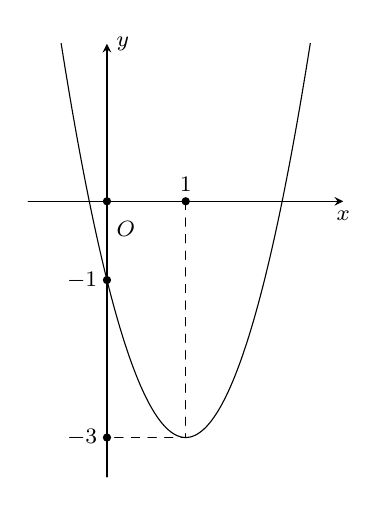
\begin{tikzpicture}[line cap=round,line join=round,>=stealth,x=1.0cm,y=1.0cm]
			\draw[->,color=black] (-1,0.) -- (3,0.) node[below] {\footnotesize $x$};
			\draw[->,color=black] (0.,-3.5) -- (0.,2) node[right] {\footnotesize $y$};
			\draw[color=black] (0pt,-10pt) node[right] {\footnotesize $O$};
			\fill (1,0) circle (1.5pt) node[above]{\footnotesize $1$}
			(0,-1) circle (1.5pt) node[left]{\footnotesize $-1$}
			(0,-3) circle (1.5pt) node[left]{\footnotesize $-3$}; 
			\draw[dashed] (1,0)--(1,-3)--(0,-3);
			\clip(-1,-3.5) rectangle (3,2);
			\draw[smooth,samples=100,domain=-1:3] plot(\x,{2*(\x)^2-4*(\x)-1});
			\fill (0cm,0cm) circle (1.5pt); 
	\end{tikzpicture}}
	\loigiai{
		Đồ thị hàm số cắt trục tung tại điểm $\left( 0;-1 \right)$ nên $c=-1$.\\
		Tọa độ đỉnh $I\left( 1;-3 \right)$ nên ta có hệ phương trình 
		$$\heva{& -\dfrac{b}{2a}=1 \\ & a\cdot 1^2+b\cdot 1-1=-3} \Leftrightarrow \heva{& 2a+b=0 \\ & a+b=-2} \Leftrightarrow \heva{& a=2 \\ & b=-4.}$$
		Vậy parabol cần tìm là $y=2x^2-4x-1$.
	}
\end{vd}

\begin{vd}%[0D3H2-3]%[Biên soạn tài liệu dạy học bộ KNTT-CS]%[Trần Xuân Hòa]
	\immini{Cho parabol $\left( P \right)\colon y=ax^2+bx+c~\left( a\ne 0 \right)$ có đồ thị như hình bên. Tính $2a+b+2c$.
	}
{\begin{tikzpicture}[line cap=round,line join=round,>=stealth,x=1cm,y=1cm]
		\draw[->] (-2,0) -- (4,0) node[below] {$x$};
		\draw[->] (0,-4.5) -- (0,1.5) node[right] {$y$};
		
		\fill (0,0) circle (1.5pt) node[below right] {$O$};
		\fill (1,0) circle (1.5pt) node[above] {$1$};
		\fill (3,0) circle (1.5pt) node[above left] {$3$};
		\fill (-1,0) circle (1.5pt) node[below left] {$-1$};
		\fill (0,-4) circle (1.5pt) node[left] {$-4$};
		
		\draw[dashed] (1,0)--(1,-4)--(0,-4);
		
		\clip(-2,-4.5) rectangle (4,1.5);
		\draw[smooth,samples=150,domain=-2:4] plot(\x,{(\x)^2-2*\x-3});
	\end{tikzpicture}
}
	\loigiai{
		Parabol $\left( P \right)\colon y=ax^2+bx+c~\left( a\ne 0 \right)$ đi qua các điểm $A\left( -1;0 \right)$, $B\left( 1;-4 \right)$, $C\left( 3;0 \right)$ nên có hệ phương trình 
		$$\heva{& a-b+c=0 \\ & a+b+c=-4 \\ & 9a+3b+c=0} \Leftrightarrow \heva{& a=1 \\ & b=-2 \\ & c=-3.}$$
		Khi đó $2a+b+2c=2\cdot 1-2+2\cdot\left( -3 \right)=-6$.
	}
\end{vd}

\begin{dang}{Ứng dụng hàm số bậc hai để giải các bài toán thực tế}
	\textbf{Phương pháp giải:} Mô hình hóa bài toán về phương trình hàm số bậc hai hoặc ứng dụng đồ thị hàm số bậc hai để giải quyết các bài toán thực tế.
\end{dang}

\begin{vd}%[0D3V2-6]%[Biên soạn tài liệu dạy học bộ KNTT-CS]%[Trần Xuân Hòa]
	\immini{
		Tại một buổi khai trương, người ta làm một cổng chào có đường viền trong của mặt cắt là đường parabol. Người ta đo khoảng cách giữa hai chân cổng là $4{,}5$ m. Từ một điểm trên thân cổng người ta đo được khoảng cách tới mặt đất là $1{,}8$ m và khoảng cách từ điểm đó tới chân cổng gần nhất là $1$ m. Hãy tính chiều cao của cổng chào đó (tính theo đường viền trong) theo đơn vị mét và làm tròn kết quả đến hàng phần mười.
	}{
		\begin{tikzpicture}[scale=1.2, font=\footnotesize, line join=round, line cap=round, >=stealth]
			\def\hso{-18/35*\x*\x+81/35*\x}
			\def\hsoo{-18/35*\x*\x+81/35*\x+.75}
			\draw[thick,blue,samples=200,smooth,fill=gray,xscale=1.2]plot[domain=0:4.5](\x,{\hso})--cycle;
			\draw[thick,blue,samples=200,smooth,fill=white,xscale=1.2]plot[domain=0:4.5](\x,{\hsoo})--cycle;
			\draw[thick,blue,samples=200,smooth,xscale=1.2]plot[domain=0:4.5](\x,{\hso})--cycle;
			\path[postaction={decorate,decoration={text color=blue,text along path,text align=center, raise=1mm,text={CH{À}O M{Ừ}NG QU{Ý} KH{Á}CH}}}] plot[domain=0:4.5,xscale=1.2] (\x,{\hso});
		\end{tikzpicture}
	}
	\loigiai{
		\immini{
			Chọn hệ trục toạ độ sao cho gốc toạ độ $O$ trùng một chân của cổng, trục hoành nằm trên đường nối hai chân cổng (đơn vị trên các trục tính theo mét). Gọi hàm số bậc hai có đồ thị chứa đường viền trong của cổng chào trên là $y = a x^2 + b x + c$ với $a\neq 0$.\\
			Từ giả thiết bài toán ta có đồ thị hàm số đi qua các điểm $O(0 ; 0)$, $ (4{,}5 ; 0)$, $ B(1 ; 1{,}8)$.
		}{
			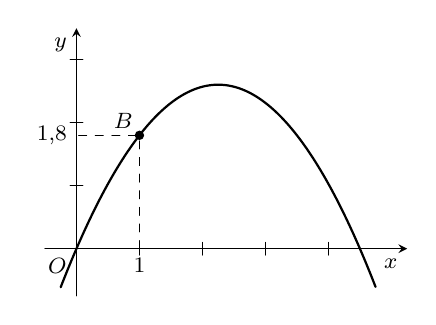
\begin{tikzpicture}[scale=0.8, font=\footnotesize, line join=round, line cap=round, >=stealth,cham/.style={circle,fill,inner sep=1.2pt}]
				\def\hso{-18/35*\x*\x+81/35*\x}
				\draw[thick,samples=200,smooth]plot[domain=-.25:4.75](\x,{\hso});
				\draw[->](-.5,0)--(5.25,0)node[below left]{$x$};
				\draw[->](0,-.75)--(0,3.5)node[below left]{$y$};
				\foreach \i in {1,...,4}{\draw (\i,.1)--(\i,-.1);}
				\foreach \i in {1,...,3}{\draw (.1,\i)--(-.1,\i);}
				\path (0,0) node[below left]{$O$};
				\draw[dashed,very thin] (1,0)node[below]{$1$}|-
				node[cham]{}node[above left=-1pt]{$B$}(0,1.8)node[left]{$1{,}8$};
			\end{tikzpicture}
		}
		Thay toạ độ các điểm trên vào hàm số, ta được hệ phương trình $$\heva{&4{,}5^{2} a + 4{,}5b = 0 \\& 1^{2} a+1 b=1{,}8\\&0=c} \Leftrightarrow \heva{&a=\dfrac{-18}{35} \\& b=\dfrac{81}{35}\\&c=0.}$$
		Suy ra ta có hàm số $y=\dfrac{-18}{35} x^2+\dfrac{81}{35} x$.\\
		Khi đó, ta có hoành độ đỉnh của đồ thị là $ x=-\dfrac{b}{2a}=\dfrac{9}{4} $.\\
		Từ đó, đỉnh của đồ thị hàm số trên có tung độ là $\dfrac{-18}{35} \cdot\left(\dfrac{9}{4}\right)^{2}+\dfrac{81}{35} \cdot \dfrac{9}{4} \approx 2,6$.\\
		Vậy chiều cao của cổng là khoảng $2{,}6$ m.
	}
\end{vd}
\begin{vd}%[0D3V2-6]%[Biên soạn tài liệu dạy học bộ KNTT-CS]%[Trần Xuân Hòa]
	Một rạp chiếu phim có sức chứa $1\ 000$ người. Với giá vé là $40\ 000$ đồng, trung bình sẽ có khoảng $300$ người đến rạp xem phim mỗi ngày. Để tăng số lượng vé bán ra, rạp chiếu phim đã khảo sát thị trường và thấy rằng nếu giá vé cứ giảm $10\ 000$ đồng thì sẽ có thêm $100$ người đến rạp mỗi ngày.
	\begin{enumerate}
		\item Tìm công thức của hàm số $R(x)$ mô tả doanh thu từ tiền bán vé mỗi ngày của rạp chiếu phim khi giá vé là $x$ nghìn đồng.
		\item Tìm mức giá vé để doanh thu từ tiền bán vé mỗi ngày của rạp là lớn nhất.
	\end{enumerate}
	\loigiai{
		\begin{enumerate}
			\item Khi giá vé là $x$ (nghìn đồng) thì số tiền giảm giá mỗi vé so với mức giá cũ là $40-x$ (nghìn đồng).\\
			Số người tăng lên sau khi giảm giá vé là $\dfrac{100(40-x)}{10}=10(40-x)$ (người).\\
			Số người đến rạp chiếu phim mỗi ngày sau khi giảm giá là
			$$300+10(40-x)=700-10x\text{ (người)}.$$
			Công thức của hàm số $R(x)$ mô tả doanh thu từ tiền bán vé mỗi ngày khi giá vé bằng $x$ (nghìn đồng) là
			$$R(x)=x(700-10x)=-10x^2+700x \text{ (nghìn đồng).}$$
			\item Hàm số $R(x)=-10x^2+700x$ là hàm số bậc hai có $ a=-10 <0 $.\\
			Đồ thị hàm số có đỉnh là $ \heva{&x_I=-\dfrac{700}{2\cdot (-10)}=35\\&y_I=-10\cdot35^2+700\cdot 35=12\,250.} $\\
			Vì $R(x)\ge 0$ nên $0\le x\le 70$.\\
			Bảng biến thiên
			\begin{center}
				
\begin{tikzpicture}[>=stealth]
					\tkzTabInit[nocadre=false,lgt=1,espcl=2,deltacl=0.5]{$x$/.7,$R(x)$/2}
					{$0$ , $35$ , $70$}
					\tkzTabVar{-/$0$ , +/$12\,250$ , -/$0$}
				\end{tikzpicture}
			\end{center}
			 Do đó hàm số đạt giá trị lớn nhất tại $x-35$ và $R(35)=12\ 250$.\\
			Vậy doanh thu lớn nhất mà rạp chiếu có thể thu được mỗi ngày là $12\ 250\ 000$ đồng khi giá bán mỗi vé là $35\ 000$ đồng.
		\end{enumerate}
	}
\end{vd}
\begin{vd}%[0D3V2-6]%[Biên soạn tài liệu dạy học bộ KNTT-CS]%[Trần Xuân Hòa]
	\immini{Hai bạn An và Bình trao đổi với nhau:
	An nói \lq\lq Tớ đọc ở một tài liệu thấy nói rằng cổng Đại học Bách Khoa Hà Nội có dạng một parabol, khoảng cách giữa hai chân cổng là $8$ m và chiều cao của cổng tính từ một điểm trên mặt đất cách chân cổng là $0{,}5$ m là $2{,}93$ m. Từ đó tớ tính ra được chiều cao của cổng parabol đó là $12$ m\rq\rq.
	Sau một hồi suy nghĩ, Bình nói \lq\lq Nếu dữ kiện như bạn nói, thì chiều cao của cổng parabol mà bạn tính ra ở trên là không chính xác\rq\rq. Dựa vào thông tin mà An đọc được, em hãy tính chiều cao của cổng Đại học Bách Khoa Hà Nội. \par\shortans{$12{,}5$}
	}
{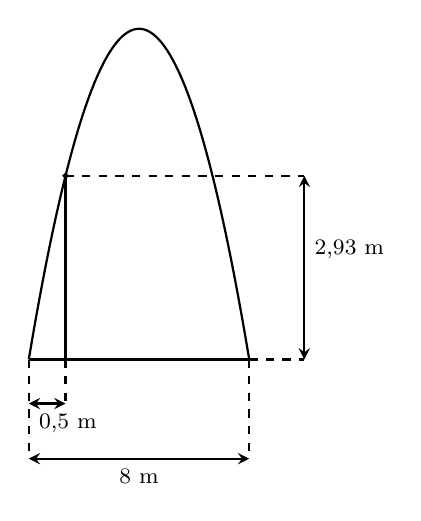
\begin{tikzpicture}[>=stealth,x=1.0cm,y=1.0cm,thick, scale=0.7]
		\draw[->] (0,-7.8) -- (2,-7.8);
		\draw[->]  (0,-7.8) -- (-2,-7.8);
		\draw[->] (-5/3,-6.8) -- (-4/3,-6.8);
		\draw[->]  (-5/3,-6.8) -- (-2,-6.8);
		\draw[->]  (3,-3) -- (3,-6);
		\draw[->]  (3,-3) -- (3,-8/3);
		\draw (3,-4) node[right] {\footnotesize $2{,}93$ m};
		\draw (0,-7.8) node[below] {\footnotesize $8$ m};
		\draw (-2,-6.8) node[below right] {\footnotesize $0{,}5$ m};
		\draw [dashed] (-4/3,-8/3)--(3,-8/3) (2,-6)--(3,-6) (2,-6)--(2,-7.8) (-2,-6)--(-2,-7.8) (-4/3,-6)--(-4/3,-6.8);
		\draw [color=black,smooth, domain=-2:2, samples=100] %
		plot (\x,{(-3/2)*(\x)^2});
		\draw (2,-6)--(-2,-6)  (-4/3,-6)--(-4/3,-8/3); 	
		\draw (-4/3,-8/3) circle (1pt);
\end{tikzpicture}}
	
	\loigiai{
		\immini{Chọn hệ trục tọa độ $Oxy$ sao cho một chân cổng đặt tại gốc tọa độ, chân còn lại đặt trên tia $Ox$.\\
		Khi đó cổng parabol là một phần của đồ thị hàm số dạng $y=ax^2+bx$ (do parabol đi qua gốc tọa độ nên hệ số tự do bằng $0$).\\
		Parabol đi qua các điểm có tọa độ $B(8; 0)$ và $A(0{,}5; 2{,}93)$.\\
		Thay tọa độ của $A$, $B$ vào hàm số ta có $$\heva{& 0=a \cdot 8^2+b \cdot 8 \\ & 2{,}93=a \cdot 0{,}5^2+b \cdot 0{,}5} \Leftrightarrow\heva{& a=\dfrac{-293}{375} \\& b=\dfrac{2\,344}{375}.}$$}
		{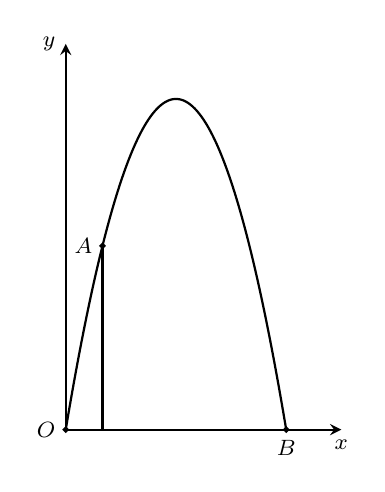
\begin{tikzpicture}[>=stealth,x=1.0cm,y=1.0cm,thick, scale=0.7]
				\draw[->] (-2,-6) -- (3,-6);
				\draw[->] (-2,-6) -- (-2,1);
				\draw [color=black,smooth, domain=-2:2, samples=100] %
				plot (\x,{(-3/2)*(\x)^2});
				\draw (2,-6)--(-2,-6)  (-4/3,-6)--(-4/3,-8/3); 	
				\draw (2,-6) node[below] {\footnotesize$B$} circle (1pt);
				\draw (-4/3,-8/3) node[left] {\footnotesize$A$} circle (1pt);
				\draw (-2,-6) node[left] {\footnotesize$O$} circle (1pt);
				\draw (-2,1) node[left] {\footnotesize$y$};
				\draw (3,-6) node[below] {\footnotesize$x$};
		\end{tikzpicture}	}
		Suy ra có hàm số $y=\dfrac{-293}{375} x^2+\dfrac{2\,344}{375} x$.\\
		Hàm số có đỉnh $I\left(4; \dfrac{4\,688}{375}\right)$ suy ra chiều cao của cổng là $\dfrac{4\,688}{375} \approx 12{,}5\mathrm{~m}$.
	}
\end{vd}

%-----------------------------------------------------------------------------
\subsection{BÀI TẬP RÈN LUYỆN}
\ind{PHẦN I.} \inden{Câu trắc nghiệm nhiều phương án lựa chọn. Mỗi câu hỏi học sinh chỉ chọn một phương án.}
\setcounter{ex}{0}
\Opensolutionfile{ans}[ans/0D3-Bai2-TN]%--Đặt tên 2D1-Bai1-Dang1-TN
\begin{ex}%[0D3N2-1]%[Biên soạn tài liệu dạy học bộ KNTT-CS]%[Trần Xuân Hòa]
	Với giá trị nào của tham số $m$ thì hàm số $y=(m+1)x^4-2x^2+2\,023$ là hàm số bậc hai?
	\choice
	{$m=0$}
	{$m=2$}
	{$m=1$}
	{\True $m=-1$}
	\loigiai{
		Hàm số  $y=(m+1)x^4-2x^2+2\,023$ là hàm số bậc hai $\Leftrightarrow m+1=0\Leftrightarrow m=-1$.
	}
\end{ex}

\begin{ex}%[0D3N2-3]%[Biên soạn tài liệu dạy học bộ KNTT-CS]%[Trần Xuân Hòa]
	Hàm số bậc hai $y=ax^2+bx+c$ có bảng biến thiên sau đây. 
		\begin{center}
			
\begin{tikzpicture}
				\tkzTabInit[lgt=1.2,espcl=3]
				{$x$/0.7,$y$/2}
				{$-\infty$,$2$,$+\infty$}
				\tkzTabVar{+/$+\infty$,-/$-5$,+/$+\infty$}
			\end{tikzpicture}
		\end{center}
		Hãy tìm tọa độ đỉnh $S$ của đồ thị hàm số đã cho.
	\choice
	{$S(5;-2)$}
	{\True $S(2;-5)$}
	{$S(-2;5)$}
	{$S(-5;2)$}
	\loigiai{
		Tọa độ đỉnh của đồ thị hàm số là $S(2;-5)$.
	}
\end{ex}

\begin{ex}%[0D3H2-1]%[Biên soạn tài liệu dạy học bộ KNTT-CS]%[Trần Xuân Hòa]
	Tìm tọa độ đỉnh $S$ của parabol $y=x^2-2x+1$.
	\choice
	{$S(0; 1)$}
	{$S(0; 0)$}
	{$S(1; 1)$}
	{\True $S(1; 0)$}
	\loigiai{
		Parabol có hoành độ đỉnh là $x=-\dfrac{b}{2a}=-\dfrac{-2}{2\cdot1}=1$.\\ Suy ra tung độ đỉnh $y=0$.\\
		Do đó tọa độ đỉnh $S(1;0)$.
	}
\end{ex}

\begin{ex}%[0D3N2-1]%[Biên soạn tài liệu dạy học bộ KNTT-CS]%[Trần Xuân Hòa]%
	Cho parabol $(P)\colon y=x^2+3x+2$. Phương trình trục đối xứng của $(P)$ là
	\choice
	{$x=-3$}
	{$y=-\dfrac{3}{2}$}
	{\True $x=-\dfrac{3}{2}$}
	{$y=-3$}
	\loigiai
	{
		Trục đối xứng của $(P)$ là $x=-\dfrac{b}{2a}=-\dfrac{3}{2}$.
	}
\end{ex}

\begin{ex}%[0D3H2-1]%[Biên soạn tài liệu dạy học bộ KNTT-CS]%[Trần Xuân Hòa]
	Cho $(P) \colon y=x^2+bx+1$ đi qua điểm $A(-1;3)$. Khi đó
	\choice
	{\True $b=-1$}
	{$b=3$}
	{$b=1$}
	{$b=-2$}
	\loigiai{
		Vì $(P)$ đi qua $A(-1;3)$ nên ta có $3=(-1)^2-b+1 \Leftrightarrow b=-1$.
	}
\end{ex}

\begin{ex}%[0D3N2-1]%[Biên soạn tài liệu dạy học bộ KNTT-CS]%[Trần Xuân Hòa]
	Cho hàm số $y=ax^2+bx+c$ có bảng biến thiên như hình dưới.
	\begin{center}
		
\begin{tikzpicture}
			\tkzTabInit
			[lgt=1.5,espcl=4] % tùy chọn
			{$x$/1, $y$/2.5} % cột đầu tiên
			{$-\infty$, $2$, $+\infty$} % hàng 1 cột 2
			\tkzTabVar{+/ $+\infty$, -/ $3$ , +/ $+\infty$} % hàng 3 cột 2
			\end{tikzpicture}
	\end{center}
	 Khẳng định nào sau đây là đúng?
	\choice
	{$a\le 0$}
	{$a\ge 0$}
	{\True $a> 0$}
	{ $a<0$}
	\loigiai{
		Dựa vào bảng biến thiên, ta thấy $a>0$.
	}
\end{ex}
\begin{ex}%[Biên soạn tài liệu dạy học bộ KNTT-CS]%[Trần Xuân Hòa]%[0D3H2-2]
	Hàm số nào sau đây đồng biến trên khoảng $(2;+\infty)$?
	\choice
	{$y=-x+4$}
	{\True $y=2x^2-8x$}
	{$y=x^2-6x+5$}
	{$y=-x^2+4x+3$}
	\loigiai{
		\immini{Xét hàm số $y=2x^2-8x$.\\
		Tọa độ đỉnh $I(2;-8)$.\\
		Bảng biến thiên như hình bên.\\
		Hàm số đã cho đồng biến trên $(2;+\infty)$ và nghịch biến trên $(-\infty;2)$.}
		{
\begin{tikzpicture}
				\tkzTabInit[nocadre=false,lgt=1.2,espcl=2.5,deltacl=0.6]
				{$x$ /0.8,$y$ /2}
				{$-\infty$,$2$,$+\infty$}
				\tkzTabVar{+/$+\infty$,-/$-8$,+/$+\infty$}
		\end{tikzpicture}}
	}
\end{ex}
\begin{ex}%[0D3N2-2]%[Biên soạn tài liệu dạy học bộ KNTT-CS]%[Trần Xuân Hòa]
	\immini{
		Hàm số nào sau đây có bảng biến thiên như hình vẽ?
		\choice
		{$y=-x^2+2 x-3$}
		{$y=x^2-2 x+3$}
		{\True $y=-x^2+2 x+1$}
		{$y=x+1$}
	}
	{
		
\begin{tikzpicture}
			\tkzTabInit[lgt=1.2,espcl=2] % tùy chọn
			{$x$/.8, $y$/2} % cột đầu tiên
			{$-\infty$, $1$, $+\infty$}
			\tkzTabVar{-/$-\infty$,+/ $2$,-/$-\infty$}
		\end{tikzpicture}
	}
	\loigiai{
		Hàm số trong bảng biến thiên là hàm số bậc hai, có hệ số $a<0$, tọa độ đỉnh $I(1;2)$.\\
		Do đó hàm số $y=-x^2+2 x+1$ thỏa mãn.
	}
\end{ex}

\begin{ex}%[0D3N2-2]%[Biên soạn tài liệu dạy học bộ KNTT-CS]%[Trần Xuân Hòa]
	Cho parabol $(P)\colon y=-x^2+4 x+5$. Phát biểu nào sau đây đúng?
	\choice
	{Giá trị lớn nhất của hàm số bằng $2$}
	{\True Giá trị lớn nhất của hàm số bằng $9$}
	{Giá trị nhỏ nhất của hàm số bằng $9$}
	{Giá trị nhỏ nhất của hàm số bằng $2$}
	\loigiai
	{
		Ta có đỉnh parabol là $I\left(2;9\right)$, $a=-1<0$ suy ra giá trị lớn nhất của hàm số bằng $9$.
	}
\end{ex}

\begin{ex}%[0D3N2-4]%[Biên soạn tài liệu dạy học bộ KNTT-CS]%[Trần Xuân Hòa]
	Biết parabol $\left(P\right)\colon y=x^2+3x+c$ cắt trục hoành tại điểm có hoành độ bằng $-5$. Tìm $c$.
	\choice
	{$c=10$}
	{$c=-5$}
	{\True $c=-10$}
	{$c=15$}
	\loigiai{
		Theo giả thiết, ta có parabol $\left(P\right)\colon y=x^2+3x+c$ cắt trục hoành tại điểm $A\left(-5;0\right)$ nên ta được
		$$ (-5)^2+3\cdot (-5)+c=0 \Leftrightarrow c=-10.$$
	}
\end{ex}

\begin{ex}%[0D3N2-4]%[Biên soạn tài liệu dạy học bộ KNTT-CS]%[Trần Xuân Hòa]
	Đồ thị của hàm số $y=x^2-3x+1$ cắt trục tung tại điểm có tọa độ là
	\choice
	{$\left(1;0\right)$}
	{$\left(0;-1\right)$}
	{\True $\left(0;1\right)$}
	{$\left(-1;0\right)$}
	\loigiai{
		Ta có $x=0$ thay vào ta được $y=1$.
	}
\end{ex}

\begin{ex}%[0D3H2-3]%[Biên soạn tài liệu dạy học bộ KNTT-CS]%[Trần Xuân Hòa]
	Đỉnh của parabol $(P)\colon y=2x^2-4x+6$ thuộc đường thẳng nào sau đây?
	\choice
	{$\Delta_1\colon y=x+4$}
	{$\Delta_2\colon y=2x+3$}
	{\True $\Delta_3\colon y=3x+1$}
	{$\Delta_4\colon y=4x-5$}
	\loigiai{
		Gọi $ I $ là đỉnh của parabol, khi đó hoành độ đỉnh là $ x_0=-\dfrac{-4}{2\cdot 2}=1 $.\\
		Tung độ đỉnh là $ y_0=2\cdot 1^2-4\cdot 1+6=4 $.\\
		Đỉnh $I(1;4)$ và tọa độ này thỏa mãn phương trình của $ \Delta_3 \colon y=3x+1$ (vì $ 4= 3\cdot 1+1 $).
	}
\end{ex}

\Closesolutionfile{ans}

\ind{PHẦN II.} \inden{Câu trắc nghiệm đúng sai. Trong mỗi ý a), b), c), d) ở mỗi câu, học sinh chọn đúng hoặc sai.}
\setcounter{ex}{0}
\Opensolutionfile{ans}[ans/0D3-Bai2-DS]%--Đặt tên 2D1-Bai1-Dang1-TN



\begin{ex}%[0D3H2-3]%[Biên soạn tài liệu dạy học bộ KNTT-CS]%[Trần Xuân Hòa]
	Cho hàm số bậc hai $y=x^2-2x-3$. Khi đó
	\choiceTF
	{\True Đồ thị hàm số nhận đường thẳng $x=1$ làm trục đối xứng}
	{Hàm số trên đồng biến trên khoảng $(-\infty;1)$ và nghịch biến trên khoảng $(1;+\infty)$}
	{Hàm số trên đạt giá trị lớn nhất trên $\mathbb{R}$ là $-4$ khi $x=1$}
	{\True Đồ thị hàm số trên là parabol có tọa độ đỉnh là $(1;-4)$}
	\loigiai{
		\begin{itemchoice}
			\itemch 
			Trục đối xứng $x=-\dfrac{b}{2a}=1$.
			\itemch 
			Vì $a=1>0$ nên hàm số trên nghịch biến trên khoảng $(-\infty;1)$ và đồng biến trên khoảng $(1;+\infty)$.
			\itemch 
			Do $a=1>0$ nên hàm số chỉ có giá trị nhỏ nhất chứ không có giá trị lớn nhất.
			\itemch 
			Hoành độ đỉnh $x=-\dfrac{b}{2a}=1$.\\
			Tung độ đỉnh $y=f(1)=1-2-3=-4$.\\
			Do đó, đồ thị hàm số trên là parabol có tọa độ đỉnh là $(1;-4)$.
		\end{itemchoice}
	}
\end{ex}
\begin{ex}%[0D3H2-1]%[KNTT-CS]%[Trần Xuân Hòa]
	Cho hàm số $y=ax^2+bx+c$, ($a\neq 0$) có đồ thị là parabol $(P)$. Khi đó
	\choiceTF
	{Nếu $(P)$ đi qua gốc tọa độ $O$ thì $b=0$}
	{Nếu $(P)$ có trục đối xứng là $x=2$ thì $4a-b=0$}
	{\True Nếu $(P)$ cắt trục hoành tại điểm có hoành độ bằng $1$ thì $a+b+c=0$}
	{\True Nếu $(P)$ có đỉnh $S(2;-3)$ và cắt trục tung tại điểm có tung độ bằng $1$ thì $a-b+c=6$}
	\loigiai{
		\begin{itemchoice}
			\itemch Nếu $(P)$ đi qua gốc tọa độ thì $$0=a\cdot0^2+b\cdot0+c\Leftrightarrow c=0.$$
			\itemch Nếu $(P)$ có trục đối xứng $x=-\dfrac{b}{2a}$ thì $$-\dfrac{b}{2a}=2\Leftrightarrow -b=4a\Leftrightarrow 4a+b=0.$$
			\itemch Nếu $(P)$ cắt trục hoành tại điểm có hoành độ bằng $1$ thì $$a\cdot 1^2+b\cdot 1+c=0\Leftrightarrow a+b+c=0.$$
			\itemch Nếu $(P)$ có đỉnh $S(2;-3)$ và cắt trục tung tại điểm có tung độ bằng $1$ thì ta có $$\heva{&4a+b=0\\&4a+2b+c=-3\\&c=1}\Leftrightarrow\heva{&a=1\\&b=-4\\&c=1.}$$
			Vậy $a-b+c=6$.
			
		\end{itemchoice}
	}
\end{ex}


\begin{ex}%[0D3V2-6]%[Biên soạn tài liệu dạy học bộ KNTT-CS]%[Trần Xuân Hòa]
	Một miếng nhôm có bề ngang $32$ cm được uốn cong tạo thành máng dẫn nước bằng cách chia tấm nhôm thành ba phần rồi gấp hai bên lại theo một góc vuông như hình vẽ dưới. Để đảm bảo kĩ thuật, diện tích mặt cắt ngang của máng dẫn nước phải lớn hơn hoặc bằng $120$ cm$^2$.\\
	\centerline
	{
		\begin{tikzpicture}[line cap=round,line join=round,font=\footnotesize,>=stealth]
			%\node[circle,shading=ball,minimum width=3cm] (ball) at (0,0) {};
			\path (0:0) coordinate(A) (0:4) coordinate(D) (60:3) coordinate(B) ($(B)+(D)-(A)$) coordinate(C) ($(A)!.3!(D)$) coordinate(E) ($(D)!.3!(A)$) coordinate(F) ($(B)!.3!(C)$) coordinate(H) ($(C)!.3!(B)$) coordinate(G);
			\fill[shading=ball,ball color=gray!30, minimum width=3cm] (A) -- (B) -- (C) --(D) -- cycle;
			\draw (A) -- (B) -- (C) -- (D) -- cycle (E)--(H) (F)--(G);
			\draw[<->] ([shift={(-90:.2)}]A) -- ([shift={(-90:.2)}]D) node[midway,below]{$32$ cm};
			\draw[<->] ([shift={(90:.1)}]B) -- ([shift={(90:.1)}]H) node[midway,above]{$x$ cm};
			\draw[<->] ([shift={(90:.1)}]G) -- ([shift={(90:.1)}]C) node[midway,above]{$x$ cm};
		\end{tikzpicture}
		\begin{tikzpicture}[line cap=round,line join=round,font=\footnotesize,>=stealth]
			\path (0:0) coordinate(A) (90:1) coordinate(B) ++(60:3) coordinate(C) ($(A)+(C)-(B)$) coordinate(D) (0:1.8) coordinate(E) ++(90:1) coordinate(H) ($(D)+(E)-(A)$) coordinate(F) ($(F)+(H)-(E)$) coordinate(G) ($(A)!.5!(D)$) coordinate(M) ++(90:1) coordinate(Q) ($(E)!.5!(F)$) coordinate(N) ++(90:1) coordinate(P);
			\fill[gray!30] (A) -- (B) --(C) -- (D) -- cycle;
			\fill[gray!60] (A) -- (D) --(F) -- (E) -- cycle;
			\fill[violet] (M) -- (N) --(P) -- (Q) -- cycle;
			\fill[green!40!black] (E) -- (F) -- (G) -- (H) -- cycle;
			\draw (A) -- (B) --(C) -- (D) -- cycle (E) -- (F) --(G) -- (H) -- cycle (A)--(E) (D)--(F);
			\draw[dashed] (M) -- (N) --(P) -- (Q) -- cycle;
			\draw[->] (E) ++(-10:1.5) node[below]{mặt cắt ngang} -- ([shift={(90:.4)}]$(M)!.5!(N)$);
			\draw[->] (C) ++(50:1.5) node[above]{chiều ngang mặt cắt} -- ([shift={(90:.05)}]$(P)!.5!(Q)$);
		\end{tikzpicture}
	}
Khi đó
	\choiceTF
	{\True Chiều ngang mặt cắt ngang của máng dẫn nước là $(32-2x)$ cm}
	{Diện tích mặt cắt ngang của máng dẫn nước là $2x(32-2x)$ cm$^2$}
	{Với $x= 5$ cm thì máng dẫn nước đảm bảo kĩ thuật}
	{\True Diện tích mặt cắt ngang của máng dẫn nước lớn nhất bằng $128$ cm$^2$}
	\loigiai
	{
		Gọi $S(x)$ là diện tích mặt cắt ngang của máng dẫn.\\
		Mặt cắt ngang là hình chữ nhật có chiều dọc là $x$ cm, chiều ngang là $(32-2x)$ cm.\\ Khi đó $S(x) = x(32-2x)$ cm$^2$, với $0<x<16$.\\
		Với $x=5$ cm thì $S(5) = 5(32-2\cdot 5) = 110<120$ nên máng dẫn nước không đảm bảo kĩ thuật.\\
		Diện tích mặt ngang lớn nhất khi hàm số $S(x)$ đạt giá trị lớn nhất trên khoảng $(0;16)$.\\
		Ta có
		\[S(x) = x(32-2x) = -2x^2+32x = -2(x-8)^2+128\leq 128, \forall x\in (0;16).\]
		Đẳng thức $S(x)=128$ xảy ra khi $x=8$.\\
		Vậy diện tích mặt cắt ngang của máng dẫn nước lớn nhất bằng $128$ cm$^2$.
		\begin{itemchoice}
			\itemch Do chiều ngang mặt cắt ngang của máng dẫn nước là $(32-2x)$ cm.
			\itemch Do diện tích mặt cắt ngang của máng dẫn nước là $x(32-2x)$ cm$^2$.
			\itemch Do $S(5) = 110<120$ nên máng dẫn nước không đảm bảo kĩ thuật.
			\itemch Do diện tích mặt cắt ngang của máng dẫn nước lớn nhất bằng $128$ cm$^2$.
		\end{itemchoice}
	}
\end{ex}

\begin{ex}%[0D3V2-6]%[KNTT-CS]%[Trần Xuân Hòa]
	Một khách sạn có $50$ phòng. Nếu mỗi phòng cho thuê với giá $400$ nghìn đồng một ngày thì toàn bộ phòng được thuê hết. Biết rằng cứ mỗi lần tăng giá lên $20$ nghìn đồng thì có thêm hai phòng bỏ trống không có người thuê. Giám đốc khách sạn muốn tăng giá thuê phòng một ngày và đã chọn giá mới để cho thuê mỗi phòng một ngày là $x$ (nghìn đồng). Khi đó
	\choiceTF
	{\True Điều kiện của $x$ là $x\ge 400$}
	{\True Giá thuê phòng chênh lệch sau khi tăng là $x-400$ (nghìn đồng)}
	{\True Số lượng phòng cho thuê giảm đi khi chọn mức giá thuê phòng mới là $\dfrac{x-400}{10}$ (phòng)}
	{Thu nhập của khách sạn trong ngày là lớn nhất khi giá thuê phòng một ngày là $x=440$ (nghìn đồng)}
	\loigiai{
		\begin{itemchoice}
			\itemch Giám đốc khách sạn muốn chọn giá mới để cho thuê phòng một ngày là $x$ (nghìn đồng). Điều kiện $x\ge 400$.
			\itemch Giá thuê phòng chênh lệch sau khi tăng là $x-400$ (nghìn đồng).
			\itemch Số lượng phòng cho thuê giảm đi khi chọn mức giá thuê phòng mới là 
			$$\dfrac{x-400}{20}\cdot 2=\dfrac{x-400}{10}~\text{(phòng)}.$$
			\itemch Số phòng cho thuê với giá $x$ là 
			$$50-\dfrac{x-400}{10}=\dfrac{900-x}{10}.$$
			Tổng thu trong ngày là 
			$$x\cdot\left( \dfrac{900-x}{10} \right)=-\dfrac{x^2}{10}+90x.$$ 
			Xét hàm số $f\left( x \right)=-\dfrac{x^2}{10}+90x$ với $x\ge 400$.\\
			Bảng biến thiên
			\begin{center}
				
\begin{tikzpicture}
					\tkzTabInit[lgt=1.5,espcl=3,deltacl=.7]
					{$x$ /.7, $f(x)$ /2.5}
					{$400$ , $450$, $+\infty$}
					\tkzTabVar{-/$20\,000$ ,+/ $20\,250$ ,-/$-\infty$}
				\end{tikzpicture}
			\end{center}
			Dựa vào bảng biến thiên ta thấy $f\left( x \right)$ đạt giá trị lớn nhất tại $x=450$.\\
			Như vậy nếu cho thuê giá $450$ nghìn đồng thì khách sạn có doanh thu cao nhất trong ngày.
		\end{itemchoice}
	}
\end{ex}
\Closesolutionfile{ans}

\ind{PHẦN III.} \inden{Câu trả lời ngắn.}
\setcounter{ex}{0}
\Opensolutionfile{ans}[ans/0D3-Bai2-TLN]%--Đặt tên 2D1-Bai1-DS
\begin{ex}%[0D3H2-3]%[KNTT-CS]%[Trần Xuân Hòa]
	Tìm $m$ để đồ thị hàm số $y=x^2-(1-m)x-3m+1$ đi qua điểm $A(1;-3)$.
	\par\shortans{$2$}
	\loigiai{
		Đồ thị hàm số $y=x^2-(1-m)x-3m+1$ đi qua điểm $A(1;-3)$ khi và chỉ khi
		\begin{center}
			$-3=1^2-(1-m)\cdot 1-3m+1 \Leftrightarrow 2m=4 \Leftrightarrow m=2$.
		\end{center}
	}
\end{ex}
\begin{ex}%[0D3H2-1]%[Biên soạn tài liệu dạy học bộ KNTT-CS]%[Trần Xuân Hòa]
	Cho parabol $(P)\colon y=ax^2+b x-4$ và trục đối xứng $x=-2$ và đi qua điểm $A\left(1;6\right)$. Tính $b-a$.
	\par\shortans[0]{$6$}
	\loigiai
	{
			Trục đối xứng $x=-2\Rightarrow-\dfrac{b}{2a}=-2\Leftrightarrow 4a-b=0$.\\
			$(P)$ đi qua điểm $A(1;6)$ nên thay $x=1$, $y=6$ vào phương trình $(P)$ suy ra \[a+b-4=6\Leftrightarrow a+b=10.\]
			Vậy ta có hệ phương trình $\heva{& 4a-b=0 \\ & a+b=10}\Leftrightarrow\heva{& a=2 \\ & b=8.}$\\
			Vậy $b-a=8-2=6$.
		}
\end{ex}

\begin{ex}%[0D3V2-4]%[Biên soạn tài liệu dạy học bộ KNTT-CS]%[Trần Xuân Hòa]
	Cho hàm số $y = f(x) = x^2 + mx + n$ ($m, n \in \mathbb{R}$) có đồ thị là parabol ($P$). Tính $ P=2m+n $ của hàm số $f(x)$ biết rằng đồ thị ($P$) cắt trục hoành tại điểm $A$ có hoành độ bằng $3$ và có trục đối xứng là đường thẳng $x = \dfrac{5}{2}$.
	\par\shortans[0]{$ -4 $}
	\loigiai{
		Ta có $x=\dfrac{-b}{2a}\Rightarrow\dfrac{5}{2}=\dfrac{-m}{2}\Rightarrow m=\dfrac{5\cdot 2}{-2}=-5$.\\
		Do ($P$) cắt trục hoành tại điểm $A$ có hoành độ bằng $3$ nên $A(3;0)\in (P) $.\\
		Suy ra $3m+n=-9\Rightarrow n=6$.\\
		Vậy $f(x)=x^2-5x+6$ nên $ P=2\cdot (-5)+6=-4$.
	}
\end{ex}


\begin{ex}%[0D3V2-6]%[Biên soạn tài liệu dạy học bộ KNTT-CS]%[Trần Xuân Hòa]
	Người quản lí của một khu chung cư có $ 200 $ căn hộ cho thuê nhận thấy rằng tất cả các căn hộ sẽ có người thuê nếu giá thuê một căn hộ là $10$ triệu đồng một tháng. Một cuộc khảo sát thị trường cho thấy rằng, trung bình cứ mỗi lần tăng giá thuê căn hộ thêm $100$ nghìn đồng thì sẽ có thêm một căn hộ bị bỏ trống. Hỏi tổng doanh thu một tháng nhiều nhất là bao nhiêu? (\textit{Đơn vị triệu đồng})
	\par\shortans[0]{$ 2\,250 $}
	\loigiai{
		Gọi số lần tăng giá tiền một phòng là $x$, $x \in \mathbb{N}$, $x \leq 200$.\\
		Khi đó giá một phòng thực tế cần cho thuê là
		$10+0{,}1x$ (triệu đồng). \\
		Số phòng thực tế thuê là $200-x$ (phòng). \\
		Vậy tổng doanh thu sẽ là $(200-x) \cdot(10+0{,}1x)=-0{,}1x^2+10x+2\,000$ (triệu đồng).\\
		Xét hàm số $f(x)=-0{,}1x^2+10x+2\,000$ với $ 0 \le x \le 200 $.\\
		Bảng biến thiên 
		\begin{center}
			% Cần khai báo \usepackage{tkz-tab}
			
\begin{tikzpicture}[>=stealth]
				\tkzTabInit[lgt=1.5,espcl=3,deltacl=.7]{$x$/.7,$y$/2.5}
				{$0$ , $50$ , $200$}
				\tkzTabVar{-/$2\,000$ , +/$2\,250$ , -/$0$}
			\end{tikzpicture}
		\end{center}
		Dựa vào bảng biến thiên, trên $ [0;200] $, hàm số $ f(x) $ có giá trị lớn nhất bằng $2\,250$ khi $x=50$.\\
		Vậy tổng doanh thu một tháng lớn nhất là $2\,250$ triệu đồng.
	}
\end{ex}

\begin{ex}%[0D3V2-6]%[Biên soạn tài liệu dạy học bộ KNTT-CS]%[Trần Xuân Hòa]
	Khi một quả bóng được ném lên, nó sẽ đạt đến độ cao nào đó rồi rơi xuống. Biết quỹ đạo của quả bóng là một cung parabol trong mặt phẳng với hệ tọa độ $Oth$, trong đó $t$ là thời gian (tính bằng giây), kể từ khi quả bóng được đá lên, $h$ là độ cao (tính bằng mét) của quả bóng. Giả thiết rằng quả bóng được đá lên từ độ cao $1{,}2$ m. Sau đó $1$ giây, nó đạt độ cao $8{,}5$ m và $2$ giây sau khi đá nó lên, nó ở độ cao $6$ m. Sau bao lâu thì quả bóng sẽ chạm đất kể từ khi đá lên \textit{(tính chính xác đến hàng phần trăm)}?
	\par\shortans[0]{$2{,}58$}
	\loigiai{
		\immini{Do bóng được đá từ độ cao $1{,}2$ m nên trong hệ trục tọa độ $Oth$ ta có parabol cắt trục $Oh$ tại điểm có tung độ $h=1{,}2$.\\
			Khi đó phương trình parabol có dạng $h(t)=at^2+bt+1{,}2$, với $t > 0$.\\
			Theo giả thiết ta có hệ phương trình\\
			$$\heva{&h(1)=a+b+1{,}2=8{,}5\\&h(2)=4a+2b+1{,}2=6}\Leftrightarrow\heva{&a+b=7{,}3\\&2a+b=2{,}4}\Leftrightarrow\heva{&a=-4{,}9\\&b=12{,}2.}$$\\
			Do đó khi quả bóng chạm đất thì độ cao của quả bóng so với mặt đất bằng $0$.\\
			Vậy $0=-4{,}9t^2+12,2t+1{,}2\Rightarrow t\approx 2{,}58$.}{
			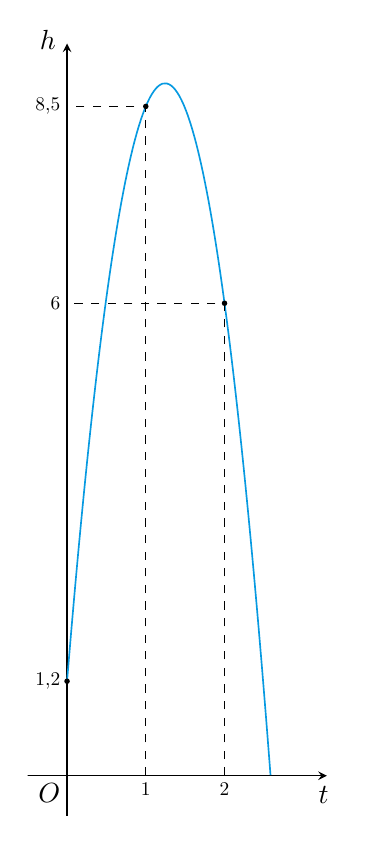
\begin{tikzpicture}[line cap=butt,line join=miter,>=stealth]
				\tikzset{declare function={xmin=-0.5-0.2;xmax=3+0.3;
						ymin=-0.5-0.2;ymax=9+0.3;
						f(\x)=- 49*(\x)^2/10 + 61*(\x)/5 + 6/5;},smooth,samples=50}
				\clip (-0.5,-0.5) rectangle (3.5,9.5);
				\draw[->] (xmin,0)--(xmax,0) node[shift={(-100:7pt)}]{$t$};
				\draw[->] (0,ymin)--(0,ymax) node[shift={(170:7pt)},font=\normalsize]{$h$};
				\fill (0,0) node[shift={(-135:9pt)}]{$O$};
				\begin{scope}
					\clip (xmin,ymin) rectangle (xmax,ymax);
					\draw[cyan!85!blue,semithick] plot[domain=0:2.584] (\x, {f(\x)});
					\fill (0,1.20) circle (1pt) node[left,,scale=.7]{$1{,}2$};
					\fill (1,8.5) circle (1pt);
					\fill (2,6) circle (1pt);
					\draw[dashed] (1,0)node[below,,scale=.7]{$1$}|-(0,8.5)node[left,scale=.7]{$8{,}5$} (2,0)node[below,,scale=.7]{$2$}|-(0,6)node[left,scale=.7]{$6$};
				\end{scope}

			\end{tikzpicture}}

	}
\end{ex}



\begin{ex}%[0D3V2-6]%[KNTT-CS]%[Trần Xuân Hòa]
	Cầu Đông Trù là một cây cầu bắc qua sông Đuống, được xây dựng theo kiểu vòm ống thép, cầu gồm $3$ nhịp chính trong đó $2$ nhịp biên dài $80$ m và nhịp giữa sông dài $120$ m. Mỗi nhịp được kiến trúc bằng đường cong tựa như một parabol.\\
	Giả sử rằng mỗi nhịp của cầu là một parabol (như hình vẽ bên dưới). Một người đã dùng dây dọi (không giãn) gắn lên thành cầu ở vị trí $B$ và điều chỉnh độ dài dây dọi để quả nặng vừa chạm đất ở vị trí $H$ (khi lặng gió). Sau đó đo được chiều dài đoạn dây dọi $BH$ là $2{,}9$ m và khoảng cách từ chân trụ cầu đến quả nặng (đoạn $OH$) là $3$ m.
	Gọi khoảng cách từ đỉnh $S$ vòm đến mặt đường là $h$. Nếu dùng dữ liệu thu thập được và tính toán thì ước tính được độ cao $h$ là bao nhiêu? (\textit{kết quả làm tròn đến hàng đơn vị}).
	\begin{center}
		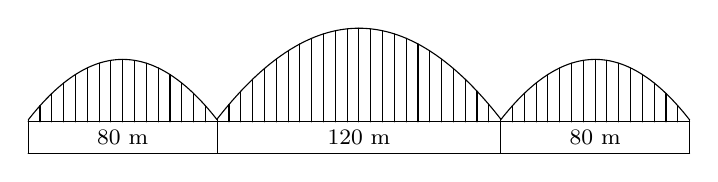
\begin{tikzpicture}[scale=.4, xscale=.75, font=\footnotesize, line join=round, line cap=round, >=stealth]
			\def\a{14}
			\pgfmathsetmacro\b{3*\a/7}
			\def\f(#1){-0.08*(#1)^2+2.97}
			\draw (-\a,0)--(\a,0) (-\a,-1)--(\a,-1);
			\foreach \i in {-\a,-\b,\b,\a} \draw (\i,0)--(\i,-1);
			\tikzset{cau/.pic={
					\draw[domain=-\b:\b, samples=100, scale=.4, xscale=.75]plot (\x, {\f(\x)});
			}}
			\tikzset{day1/.pic={
					\foreach \m in {-6,-5.5,...,6} \draw[scale=.4, xscale=.75] (\m,{\f(\m)})--(\m,0);
			}}
			\tikzset{day2/.pic={
					\foreach \m in {-6,-5.25,...,6} \draw[scale=.4, xscale=.75] (\m,{\f(\m)})--(\m,0);
			}}
			\draw (0,0) pic{cau} pic{day1};
			\draw (-10,0) pic[scale=2/3]{cau} pic[scale=2/3]{day2};
			\draw (10,0) pic[scale=2/3]{cau} pic[scale=2/3]{day2};
			\draw (0,-0.5) node{$120$ m} (-10,-0.5) node{$80$ m} (10,-0.5) node{$80$ m};
		\end{tikzpicture}
	\end{center}

	\begin{center}
		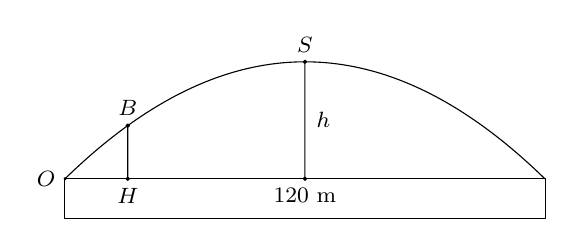
\begin{tikzpicture}[scale=.5, font=\footnotesize, line join=round, line cap=round, >=stealth]
			\def\a{14}
			\pgfmathsetmacro\b{3*\a/7}
			\def\f(#1){-0.08*(#1)^2+2.97}
			\tikzset{cau/.pic={
					\draw[domain=-\b-0.1:\b+0.1, samples=100, scale=.5]plot (\x, {\f(\x)});
			}}
			\draw (0,0) pic{cau};
			\draw (-\b-0.1,0)--(-\b-0.1,-1)--(\b+0.1,-1)--(\b+0.1,0)--cycle;
			\draw (-4.5,{\f(-4.5)}) node[above]{$B$}circle (1.2pt) -- (-4.5,0) node[below]{$H$} circle (1.2pt)
			(0,2.97) node[above]{$S$}circle (1.2pt)-- (0,0)circle (1.2pt);
			\fill[black] (-6.09,0) node[left]{$O$}circle (1.2pt) (0.05, 1.5) node[right]{$h$} (0,0)node[below]{$120$ m};
		\end{tikzpicture}

	\end{center}
	\par\shortans[0]{$30$}
	\loigiai{
		\immini{Chọn hệ trục tọa độ $O'xy$.\\
		Theo giả thiết $BH=2{,}9$ m; $OH=3$ m.\\
		Gọi $(P)\colon y=ax^2+c$ $(a<0)$ do trục đối xứng $x=0$ nên $b=0$. Cần xác định tọa độ đỉnh $S$ hay tìm $c$.\\
		Dễ thấy $O(-60;0)$, $H(-57;0)$, $B(-57;2{,}9)$.\\
		Do $O$, $B\in (P)$ ta có hệ phương trình
		$$\heva{&3\,600a+c=0 &\\&3\,249a+c=2{,}9&}\Leftrightarrow \heva{&a=-\dfrac{29}{3\,510}&\\
			&c=\dfrac{1\,160}{39}\approx 29{,}7436.&}$$
		Vậy độ cao $h=30$ m.}
		{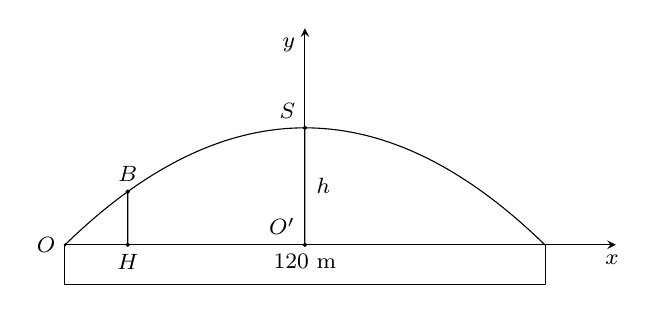
\begin{tikzpicture}[scale=.5, font=\footnotesize, line join=round, line cap=round, >=stealth]
				\def\a{14}
				\pgfmathsetmacro\b{3*\a/7}
				\def\f(#1){-0.08*(#1)^2+2.97}
				\tikzset{cau/.pic={
						\draw[domain=-\b-0.1:\b+0.1, samples=100, scale=.5]plot (\x, {\f(\x)});
				}}
				\draw (0,0) pic{cau};
				\draw (-\b-0.1,0)--(-\b-0.1,-1)--(\b+0.1,-1)--(\b+0.1,0)--cycle;
				\draw (-4.5,{\f(-4.5)}) node[above]{$B$}circle (1.2pt) -- (-4.5,0) node[below]{$H$} circle (1.2pt)
				(0,2.97) node[above left]{$S$}circle (1.2pt)-- (0,0)circle (1.2pt);
				\fill[black] (-6.09,0) node[left]{$O$}circle (1.2pt) (0.05, 1.5) node[right]{$h$} (0,0)node[below]{$120$ m};
				\draw [->] (-3.5,0)--(7.9,0);
				\draw [->] (0,0)--(0,5.5);
				\draw (0,0) node[above left]{$O'$};
				\draw (7.8,0) node[below]{$x$};
				\draw (0,5.5) node[below left]{$y$};
				%	\draw (0,1) node[above right]{$1$};
		\end{tikzpicture}}
	}
\end{ex}



\Closesolutionfile{ans}

\ind{PHẦN IV.} \inden{Tự luận.}
\setcounter{ex}{0}
\begin{ex}%[0D3H2-2]%[KNTT-CS]%[Trần Xuân Hòa]
	Gọi $M$ và $m$ lần lượt là giá trị lớn nhất và giá trị nhỏ nhất của hàm số $y=-x^2+4 x+3$ trên đoạn $[0 ; 5]$. Khi đó $m+M$ bằng
	\loigiai{
		Ta có hàm số $ y=-x^2+4x+3 $ là hàm số bậc hai.\\
		Suy ra đồ thị hàm số là đường parabol có đỉnh là $ I(2;7)$.\\
		Do $ a=-1<0 $ nên bề lõm hướng xuống, ta có bảng biến thiên của hàm số trên $ [0;5] $ như sau
		\begin{center}
			
\begin{tikzpicture}[>=stealth]
				\tkzTabInit[nocadre=false,lgt=1,espcl=2,deltacl=0.5]{$x$/.7 ,$y$/2}
				{$0$ , $2$ , $5$}
				\tkzTabVar{-/$3$ , +/$7$ , -/$-2$}
			\end{tikzpicture}
		\end{center}
	Giá trị lớn nhất trên $[0;5]$ bằng $M=7$ khi $x=2$.\\
	Giá trị nhỏ nhất trên $[0;5]$ bằng $m=-2$ khi $x=5$.\\
	Khi đó $M+m=7-2=5$.
	}
\end{ex}

\begin{ex}%[0D3H2-1]%[KNTT-CS]%[Trần Xuân Hòa]
	Xác định giá trị $a$ và $b$ để đồ thị $(P)$ của hàm số $y=ax^2+bx+5$ có đỉnh $S(2;-3)$.
	\loigiai{Theo giả thiết, ta có
		\begin{eqnarray*}
			\heva{&S\in (P)\\&x_S=2}\Leftrightarrow \heva{&4a+2b+5=-3\\&-\dfrac{b}{2a}=2}\Leftrightarrow\heva{&4a+2b=-8 \\ &4a+b=0}\Leftrightarrow \heva{&a=2\\&b=-8.}
		\end{eqnarray*}
		Vậy $(P)\colon y=2x^2-8x+5$.}
\end{ex}

\begin{ex}%[0D3H2-1]%[KNTT-CS]%[Trần Xuân Hòa]
	\immini{Tìm công thức của hàm số bậc hai  có đồ thị như hình bên.}
	{\begin{tikzpicture}[>=stealth,line join=round,line cap=round,font=\footnotesize,scale=.8]
			\draw[->] (-2.5,0)--(4,0)node[below]{$x$};
			\draw[->] (0,-2.2)--(0,4.5)node[right]{$y$};
			\draw (0,0) node[below right] {$O$};
			\fill (-1,0)circle(0.03)node[above left]{$-1$}
			(3,0)circle(0.03)node[below]{$3$}
			(0,4)circle(0.03)node[left]{$4$}
			(1,0)circle(0.03)node[below]{$1$}
			(0,3)circle(0.03)node[left]{$3$};
			\draw[ domain=-1.5:3.5, samples=100] plot (\x,{-(\x)^2+2*\x+3});
			\draw[dashed] (1,0)|-(0,4);
	\end{tikzpicture}}
	\loigiai{
		Hàm số cần tìm có dạng $y=ax^2+bx+c$ với $a<0$.\\
		Đồ thị hàm số đi qua $(-1;0)$, $(3;0)$, $(0;3)$ và $(1;4)$ nên
		$$\heva{&a-b+c=0\\&9a+3b+c=0\\&c=3\\&a+b+c=4}\Leftrightarrow \heva{&a=-1\\&b=2\\&c=3.}$$
		Vậy hàm số cần tìm là $y=-x^2+2x+3$.	}
\end{ex}

\begin{ex}%[0D3V2-6]%[KNTT-CS]%[Trần Xuân Hòa]
	Một doanh nghiệp tư nhân A chuyên kinh doanh xe gắn máy các loại. Hiện nay doanh nghiệp đang tập trung chiến lược vào kinh doanh xe Honda Future Fi với chi phí mua vào một chiếc là $27$ (triệu đồng) và bán ra với giá là $31$ triệu đồng. Với giá bán này thì số lượng xe mà khách hàng sẽ mua trong một năm là $600$ chiếc. Nhằm mục tiêu đẩy mạnh hơn nữa lượng tiêu thụ dòng xe đang ăn khách này, doanh nghiệp dự định giảm giá bán và ước tính rằng nếu giảm $1$ triệu đồng mỗi chiếc xe thì số lượng xe bán ra trong một năm là sẽ tăng thêm $200$ chiếc. Vậy doanh nghiệp phải định giá bán mới là bao nhiêu để sau khi đã thực hiện giảm giá, lợi nhuận thu được sẽ là cao nhất?
	\loigiai{
		Gọi $x$ (triệu đồng) là số tiền mà doanh nghiệp A dự định giảm giá $\left( 0\le x\le 4 \right)$.\\
		Khi đó lợi nhuận thu được khi bán một chiếc xe là $31-x-27=4-x$ (triệu đồng).\\
		Số xe mà doanh nghiệp sẽ bán được trong một năm là $600+200x$ (chiếc).\\
		Lợi nhuận mà doanh nghiệp thu được trong một năm là
		$$f\left( x \right)=\left( 4-x \right)\left( 600+200x \right)=-200x^2+200x+2\,400.$$
		Hàm số $f\left( x \right)=-200x^2+200x+2\,400$ trên đoạn $\left[0;4 \right]$ có bảng biến thiên
		\begin{center}
			
\begin{tikzpicture}
				\tkzTabInit[nocadre=false,lgt=1.2,espcl=2.5,deltacl=0.6]
				{$x$ /1,$y$ /2}
				{$0$,$\dfrac{1}{2}$,$4$}
				\tkzTabVar{-/$2\,400$, +/$2\,450$,-/$0$}
			\end{tikzpicture}
		\end{center}
		Vậy $\underset{\left[0;4 \right]}{\mathop{\max}}f\left( x \right)=2\,450\Leftrightarrow x=\dfrac{1}{2}$.\\
		Vậy giá mới của chiếc xe là $31-0{,}5=30{,}5$ triệu đồng thì lợi nhuận thu được là cao nhất.}%<MyLT2>
\end{ex}
\begin{ex}%[0D3V2-6]%[KNTT-CS]%[Trần Xuân Hòa]
	Nhân dịp Tết sắp đến, một cửa hàng bán đồ lưu niệm dự định thiết kế hàng loạt các sản phẩm bằng kính dày $5$ mm có khắc hình cành mai lên bề mặt như hình $1$. Trước khi đi vào sản xuất, cửa hàng đã dự trù chi phí dựa trên việc tính toán diện tích một mặt $S$ của mỗi tấm kính theo công thức như hình $2$. Biết rằng viền của tấm kính là một phần đồ thị của hàm số bậc hai như hình $3$. Tính chi phí kính tối thiểu để làm một sản phẩm biết mỗi mét vuông kính dày $5$ mm có giá $220\,000$ đồng, bỏ qua sự hao hụt trong quá trình cắt kính \textit{(làm tròn kết quả đến hàng đơn vị)}.
	\begin{center}
		\begin{tabular}{c c c}
			\definecolor{green(pigment)}{rgb}{0.0, 0.65, 0.31}
			\definecolor{canaryyellow}{rgb}{1.0, 0.94, 0.0}
			\definecolor{gold}{rgb}{1.0, 0.84, 0.0}
			\definecolor{cadmiumred}{rgb}{0.89, 0.0, 0.13}
			\definecolor{brown(traditional)}{rgb}{0.59, 0.29, 0.0}
			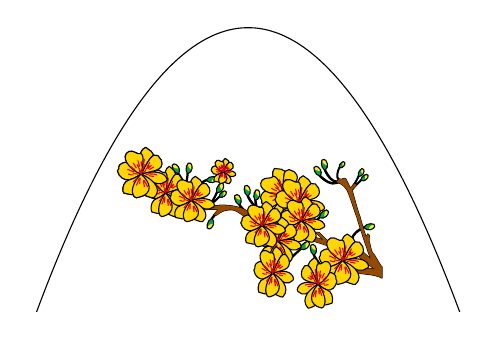
\begin{tikzpicture}[line join=round, line cap=round,scale=0.2,transform shape]
				\clip (-14,-6) rectangle (14,12);

				\tikzset{than/.pic={
						\def\Canh{
							(8.5,-3.2)
							..controls +(140:.2) and +(-40:.2) ..(7.9,-2.3)
							..controls +(150:.1) and +(-60:.1) ..(7.68,-1.58)
							..controls +(130:.1) and +(-80:.1) ..(7.7,-1.2)--(7.6,-1.1)--(7.5,-1.3)
							..controls +(130:.1) and +(-80:.1) ..(7.1,0)
							..controls +(130:.1) and +(-80:.1) ..(6.6,1.7)--(6.9,2)--(6.75,2.1)--(6.5,1.8)--(6.2,2.4)
							..controls +(140:.2) and +(-40:.2) ..(5.8,2.4)--(5.6,2.2)
							..controls +(-10:.2) and +(120:.2) ..(6.2,1.8)
							..controls +(-30:.2) and +(120:.2) ..(6.9,0)
							..controls +(-80:.2) and +(120:.2) ..(7.8,-2.7)
							..controls +(140:.2) and +(-50:.2) ..(6.6,-1.6)--(6.4,-1.6)--(6.6,-1.85)
							..controls +(160:.2) and +(-30:.2) ..(5,-1.5)--(4.5,-1)--(4.3,-1)--(4.8,-1.5)
							..controls +(160:.2) and +(-40:.5) ..(0,.3)
							..controls +(140:.6) and +(10:.5) ..(-2,.7)
							..controls +(-170:.6) and +(10:.5) ..(-4,.5)--(-4,.3)
							..controls +(10:.6) and +(160:.2) ..(-1.9,.45)--(-2.2,.1)--(-2,.1)
							..controls +(40:.6) and +(140:.6) ..(-.5,.2)
							..controls +(-40:1) and +(155:.8) ..(7,-2.5)
							..controls +(-40:.4) and +(155:.4) ..(8.2,-3.4)
							..controls +(150:.4) and +(-40:.2) ..(7,-3.2)--(6.8,-3.5)
							..controls +(-30:.4) and +(150:.6) ..(8.5,-3.9)--cycle

							;
						}
						\draw[black]\Canh;
						\fill[brown(traditional)] \Canh;
				}}

				\tikzset{bup1/.pic={
						\def\B1{
							(5.2,1.8)
							..controls +(-155:.1) and +(-50:.1) ..(4.6,2.6)
							..controls +(60:.3) and +(0:.2) ..(4.3,3.2)
							..controls +(-180:.3) and +(180:.2) ..(4.5,2.6)
							..controls +(-50:.5) and +(140:.1) ..(5,1.8)--cycle

							;
						}
						\fill[green(pigment)] \B1;

						\def\b1{
							(4.62,2.9)
							..controls +(65:.1) and +(0:.1) ..(4.3,3.2)
							..controls +(-180:.2) and +(180:.5) ..cycle
							;
						}
						\fill[canaryyellow] \b1;
						\draw[black]\B1;
				}}

				\tikzset{bup/.pic={
						\def\B{
							(5.6,2.2)
							..controls +(-155:.4) and +(-40:.4) ..(4.6,2.6)
							..controls +(60:.3) and +(0:.2) ..(4.3,3.2)
							..controls +(-180:.3) and +(180:.2) ..(4.5,2.6)
							..controls +(-50:.5) and +(-155:.3) ..(5.6,2.1)
							..controls +(25:.1) and +(-155:.1) ..(5.9,2.2)--cycle
							;
						}
						\fill[green(pigment)] \B;

						\def\b{
							(4.62,2.9)
							..controls +(65:.1) and +(0:.1) ..(4.3,3.2)
							..controls +(-180:.2) and +(180:.5) ..cycle
							;
						}
						\fill[canaryyellow] \b;
						\draw[black]\B;
				}}

				\tikzset{mai/.pic={
						\def\D{
							(-6.8,2.7)
							..controls +(80:.2) and +(-160:.7) ..(-6.5,4.4)
							..controls +(-30:.1) and +(150:.1) ..(-6.3,4.25)
							..controls +(0:.1) and +(120:.2) ..(-6,3.9)
							..controls +(-150:.4) and +(50:.2) ..cycle
							(-6.8,2.7)
							..controls +(20:.5) and +(120:.5) ..(-5.2,2.5)
							..controls +(-60:.3) and +(30:.3) ..(-5.5,2.1)
							..controls +(-150:.05) and +(30:.05) ..(-5.65,2.1)
							..controls +(-150:.05) and +(30:.05) ..(-5.8,2.1)
							..controls +(160:.8) and +(-35:.5) ..cycle
							(-6.8,2.7)
							..controls +(-150:.4) and +(10:.2) ..(-7.5,2.35)
							..controls +(-170:.4) and +(-75:.4) ..(-8.3,2.9)
							..controls +(40:.1) and +(-85:.1) ..(-8.2,3.2)
							..controls +(95:.1) and +(175:.1) ..(-7.8,3.45)
							..controls +(-5:.4) and +(145:.4) ..cycle
							;
						}
						\fill[gold] \D;
						\draw[black]\D;
						\def\C{

							(-6,3.9)
							..controls +(-150:.4) and +(50:.2) ..(-6.8,2.7)
							..controls +(20:.6) and +(-70:.8) ..(-5.52,3.6)
							..controls +(95:.05) and +(-30:.05) ..(-5.6,3.7)
							..controls +(95:.2) and +(0:.2) ..cycle

							(-6.8,2.7)
							..controls +(-20:.6) and +(40:.9) ..(-6,1.2)
							..controls +(-140:.1) and +(-10:.1) ..(-6.7,1.4)
							..controls +(170:.1) and +(-40:.1) ..cycle

							(-6.8,2.7)
							..controls +(-90:.6) and +(20:.6) ..(-7.3,1.4)
							..controls +(-160:.1) and +(-10:.1) ..(-7.9,1.5)
							..controls +(130:.1) and +(-80:.1) ..(-7.95,1.65)
							..controls +(100:.2) and +(-170:.4) ..(-7.5,2.35)
							..controls +(10:.2) and +(-150:.4) ..cycle

							(-6.8,2.7)
							..controls +(160:.8) and +(-155:.7) ..(-7.55,4.15)
							..controls +(-15:.3) and +(155:.7) ..(-7,4)
							..controls +(30:.1) and +(150:.1) ..(-6.8,4)
							..controls +(-30:.3) and +(80:.3) ..cycle
							;
						}

						\fill[gold] \C;
						\draw[black]\C;

						\def\T{
							(-6.8,2.7)
							..controls +(-40:.65) and +(10:1.3) ..(-7.1,1.2)
							..controls +(-170:.1) and +(-110:.05) ..(-7.3,1.4)
							..controls +(120:.4) and +(-140:.4) ..cycle
							;
						}
						\fill[gold] \T;
						\draw[black]\T;
						%============
						\def\V{
							(-6.8,2.7)
							..controls +(30:.1) and +(-130:.1) ..(-6.7,2.9)
							(-6.8,2.7)
							..controls +(30:.1) and +(-130:.1) ..(-6.8,3)
							(-6.8,2.7)
							..controls +(120:.1) and +(-30:.1) ..(-6.9,2.94)
							(-6.8,2.7)
							..controls +(150:.1) and +(-40:.1) ..(-6.9,2.85)
							;
						}
						\draw[cadmiumred]\V;
						%\fill[ecru!80] \V;
						%=================
						\def\N{
							(-7.3,3.4)
							..controls +(-40:.05) and +(140:.05) ..(-7.1,3.1)
							(-7.05,3.3)
							..controls +(-40:.05) and +(120:.05) ..(-6.9,3)
							(-7,3.55)
							..controls +(-40:.05) and +(120:.05) ..(-6.9,3.2)
							(-6.8,3.5)
							..controls +(-40:.05) and +(120:.05) ..(-6.75,3.2)
							(-6.6,3.3)
							..controls +(-40:.05) and +(100:.05) ..(-6.7,3)
							(-6.6,3.65)
							..controls +(-40:.05) and +(100:.05) ..(-6.65,3.3)
							(-6.3,3.25)
							..controls +(-40:.05) and +(100:.05) ..(-6.5,3)
							(-6.25,3.45)
							..controls +(-40:.05) and +(100:.05) ..(-6.4,3.2)
							(-6.35,3.05)
							..controls +(40:.05) and +(-150:.05) ..(-6.15,3.25)
							(-6.25,3)
							..controls +(40:.05) and +(-150:.05) ..(-6,3.15)
							(-6.3,2.6)
							..controls +(40:.05) and +(-150:.05) ..(-6,2.55)
							(-7.3,2.75)
							..controls +(40:.05) and +(-150:.05) ..(-7,2.7)
							(-7.6,2.7)
							..controls +(-40:.05) and +(-150:.05) ..(-7.3,2.65)
							(-7.65,3)
							..controls +(10:.05) and +(-150:.05) ..(-7.25,2.85)
							(-7.5,3.2)
							..controls +(10:.05) and +(-150:.05) ..(-7.2,3)
							(-7.3,2.2)
							..controls +(10:.05) and +(-150:.05) ..(-7.1,2.4)
							(-7.1,2)
							..controls +(10:.05) and +(-150:.05) ..(-6.9,2.45)
							(-6.9,2.1)
							..controls +(10:.05) and +(-150:.05) ..(-6.85,2.45)
							(-6.6,1.9)
							..controls +(10:.05) and +(-150:.05) ..(-6.65,2.3)
							(-6.4,1.9)
							..controls +(10:.05) and +(-150:.05) ..(-6.58,2.3)
							(-6.2,2.75)
							..controls +(-150:.05) and +(20:.05) ..(-6.5,2.65)
							(-6.2,2.7)
							..controls +(30:.05) and +(120:.05) ..(-5.8,2.65)
							(-6.65,2.8)
							..controls +(30:.05) and +(-100:.05) ..(-6.5,2.95)
							;
						}
						\draw[cadmiumred]\N;
				}}

				\path
				(0,0)pic[scale=1]{bup}
				(3.4,4.7)pic[scale=.8,rotate=-60]{bup1}
				(4.5,5.55)pic[scale=.8,rotate=-80]{bup1}
				(-.3,2.1)pic[scale=1,rotate=-20]{bup}
				(3,5.5)pic[scale=.7,rotate=-70]{bup}
				(-4.7,2)pic[scale=1,rotate=-40]{bup}
				(-5.5,-1)pic[scale=1,rotate=-10]{bup}
				(-5.2,.45)pic[scale=1,rotate=-20]{bup}
				(-7.25,1.62)pic[yscale=-1,scale=1,rotate=-10]{bup}
				(-6.5,4.2)pic[scale=1,rotate=-60]{bup1}
				(-9,3.7)pic[scale=1,rotate=-40]{bup1}
				(-9,.15)pic[scale=1]{bup1}
				(0,2)pic[scale=1,rotate=-80]{bup1}
				(1.2,4)pic[scale=1,rotate=-80]{bup1}
				(-1,-3.3)pic[scale=1,rotate=-20]{bup}
				(-3.5,7.5)pic[scale=1,rotate=-110]{bup}
				(6.5,4.5)pic[scale=1,rotate=-110]{bup}
				(-4.5,4.5)pic[scale=.8,rotate=-80]{bup1}
				;
				\path (0,0)pic[scale=1]{than}
				(0,0)pic[scale=1]{mai}
				(1.8,1.5)pic[scale=.5]{mai}
				(.2,-1.2)pic[xscale=.8]{mai}
				(0,0)pic[scale=1]{mai}
				(2.5,-1.4)pic[scale=.9]{mai}
				(9.5,2.5)pic[scale=1,rotate=30]{mai}
				(10,-1.8)pic[scale=1]{mai}
				(9.5,-2.7)pic[scale=.9]{mai}
				(8,-4)pic[scale=.9]{mai}
				(7,-3)pic[scale=.9]{mai}
				(7,-6.3)pic[xscale=.8]{mai}
				(12.8,-5.5)pic[scale=1]{mai}
				(-1,-7)pic[xscale=-.8,rotate=0]{mai}

				;
				\draw[smooth,samples=100,domain=-14:14] plot(\x,{-.1*(\x)^2+12});
				%\draw (12,8) node[above] {Hình 1};
			\end{tikzpicture}
			&
			\begin{tikzpicture}[scale=0.7, font=\footnotesize, line join=round, line cap=round, >=stealth]
				\def\xmin{-4}\def\xmax{4}\def\ymin{0}\def\ymax{6}
				\draw[<->] (2,0)--(2,4) node[midway, right] {\footnotesize $h$};
				\draw[<->] (0,0)--(4,0) node[midway, below] {\footnotesize $d$};
				\clip (-0.5,0) rectangle (4.2,6);
				\draw[smooth,samples=200,domain=\xmin:\xmax] plot (\x,{-1*((\x)^2)+4*(\x)});
				\draw (2,5.5) node[below] {$S=\dfrac{2}{3}hd$};
				%\draw (3,0.2) node[above] {Hình 2};
			\end{tikzpicture}
			&
			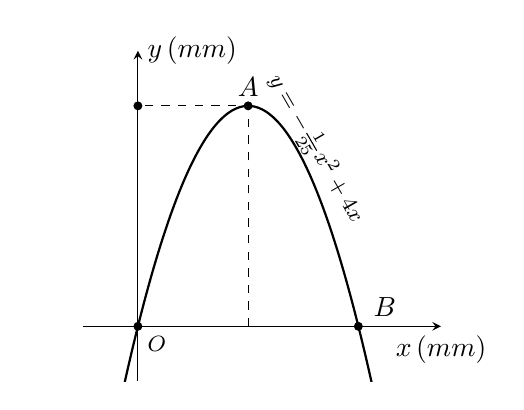
\begin{tikzpicture}[>=stealth,x=1cm,y=1cm,scale=0.7]
				\def\a{-1}
				\def\d{4}
				\def\b{-0.5}
				\def\c{1}
				\draw[->] (-1,0)--(5.5,0)node[below]{$x\left(\text{mm}\right)$};
				\draw[->] (0,-1)--(0,5)node[right]{$y\left(\text{mm}\right)$};
				\draw (0,0)node[below right]{\footnotesize $O$};
				\clip (-2,-1) rectangle(5.2,5);
				\draw[thick,samples=150,smooth,domain=-5:5] plot(\x,{\a*(\x)^2+\d*(\x)});
				\draw [dashed] (2,0)--(2,4)--(0,4);
				\draw (2,4) node[above]{$A$};
				\draw (2.85,3) node[above,rotate=-60]{\footnotesize $y=-\frac{1}{25}x^2+4x$};
				\fill (4.1,0) node[above right]{$B$};
				\foreach \x/\y in {0/0,0/4,2/4,4/0}{\draw[fill=black] (\x,\y) circle (2pt);}
				%\fill (2,-1) node[below] {Hình 3};
			\end{tikzpicture}\\
			Hình 1 & Hình 2 & Hình 3
		\end{tabular}
	\end{center}
	\loigiai{
		Phương trình $-\dfrac{1}{25}x^2+4x=0\Leftrightarrow\hoac{&x=0\\&x=100}$ nên tọa độ điểm $B\left(100;0\right)$, tức $d=100$ mm.\\
		Tọa độ đỉnh của parabol là $A\left(50;100\right)$  nên $h=100$ mm.\\
		Vậy diện tích của mỗi tấm kính là $\dfrac{2}{3}\cdot100\cdot100 = \dfrac{20\,000}{3}$ mm$^2$  $= \dfrac{1}{150} $m$^2$.\\
		Chi phí sản xuất một tấm kính là $\dfrac{1}{150}\cdot220\,000\approx1\,467$ đồng.
	}
\end{ex}
\begin{ex}%[0D3C2-6]%[KNTT-CS]%[Trần Xuân Hòa]
	Chiếc cầu dây văng một nhịp được thiết kế hai bên thành cầu có dạng parabol và được cố định bằng các dây cáp song song.
	\begin{center}
		\begin{tikzpicture}[scale=0.7,>=stealth, font=\footnotesize, line join=round, line cap=round]  
			\draw[thick] (-10,0)--(10,0)node[below left]{};
			%	\draw[->] (0,-1.2)--(0,1.7)node[left]{$y$};
			\draw[samples=100,domain=-10:10] plot (\x,{0.02*(\x)^2+1});
			\foreach \i in {-10,-9,-8,-7,-6,-5,-4,-3,-2,-1,0,1,2,3,4,5,6,7,8,9,10}{\draw(\i,0) circle (1pt)  node[scale=1]{};}
			\foreach \x in {-10,-9,-8,-7,-6,-5,-4,-3,-2,-1,0,1,2,3,4,5,6,7,8,9,10}{\draw (\x,0)--(\x,{0.02*(\x)^2+1});}
			\draw[thick] (-8.7,2)--(11.3,2)node[below left]{};
			\foreach \i in {-8.7,-7.7,-6.7,-5.7,-4.7,-3.7,-2.7,-1.7,-0.7,0.3,1.3,2.3,3.3,4.3,5.3,6.3,7.3,8.3,9.3,10.3,11.3}{\draw(\i,2) circle (1pt)  node[scale=1]{};}
			\draw[thick] (-8.7,2)--(11.3,2)node[below left]{};
			\filldraw[draw, pattern = north east lines](-10,0)--(-8.7,2)--(11.3,2)--(10,0)--cycle;
			\draw[samples=100,domain=-8.7:11.3] plot (\x,{0.02*(\x)^2+3});
			\foreach \x in {-8.7,-7.7,-6.7,-5.7,-4.7,-3.7,-2.7,-1.7,-0.7,0.3,1.3,2.3,3.3,4.3,5.3,6.3,7.3,8.3,9.3,10.3,11.3}{\draw (\x,2)--(\x,{0.02*(\x)^2+3});}
			\draw (0,-0.5)node[below left]{$\text{Hình vẽ cầu dây văng}$};
		\end{tikzpicture}
		
		\begin{tikzpicture}[scale=0.7,>=stealth, font=\footnotesize, line join=round, line cap=round]  
			\draw[thick] (-10,0)--(10,0)node[below left]{};
			\draw[samples=100,domain=-10:10] plot (\x,{0.02*(\x)^2+1});
			\foreach \i in {-10,-9,-8,-7,-6,-5,-4,-3,-2,-1,0,1,2,3,4,5,6,7,8,9,10}{\draw(\i,0) circle (1pt)  node[scale=1]{};}
			\foreach \x in {-10,-9,-8,-7,-6,-5,-4,-3,-2,-1,0,1,2,3,4,5,6,7,8,9,10}{\draw (\x,0)--(\x,{0.02*(\x)^2+1});}
			\draw[->] (0,-0.5)--(10,-0.5)node[left]{};
			\draw[->] (0,-0.5)--(-10,-0.5)node[left]{};
			\draw (5,-0.7)node[below left]{$30m$};
			\draw (0,-1)node[below left]{$\text{Hình chiếu đứng của cầu dây văng}$};
			
			\draw[->] (0,-0.5)--(10,-0.5)node[left]{};
			\draw[->] (0,-0.5)--(-10,-0.5)node[left]{};
			
			\draw[->] (10.2,0.5)--(10.2,3)node[left]{};
			\draw[->] (10.2,0.5)--(10.2,0)node[left]{};
			\draw (10.5,1)node[below right]{$5m$};
			\draw[->] (0,-0.5)--(-10,-0.5)node[left]{};
			
			\draw[->] (-10.2,0.5)--(-10.2,3)node[left]{};
			\draw[->] (-10.2,0.5)--(-10.2,0)node[left]{};
			\draw (-10.5,1)node[below left]{$5m$};
			
			\draw (1,3)node{$0{,}8m$};
			\draw[->] (1,2.5)--(0,0.5)node[left]{};
		\end{tikzpicture}
	\end{center}
	Dựa vào bản vẽ ở hình chiếu đứng của cầu dây văng, hãy tính chiều dài tổng cộng của các dây cáp dọc ở hai mặt bên, biết dây dài nhất là $5$ mét, dây ngắn nhất là $0{,}8$ mét. Khoảng cách giữa các dây bằng nhau.
	Nhịp cầu dài $30$ mét. Cần tính thêm $5\%$ chiều dài mỗi sợi dây cáp để neo cố định.
	\loigiai{
		Gọi $y=ax^2+bx+c$ là công thức của hàm số có đồ thị là thành cầu.\\
		Khi đó độ dài dây cáp dọc ở mỗi mặt bên là tung độ của điểm biểu diễn tương ứng.\\
		Ở mỗi mặt có $21$ dây cáp dọc tương ứng cho $20$ khoảng cách giữa chúng.\\
		Khoảng cách giữa hai dây cáp liền kề là $30:20=1{,}5$ mét\\
		Khi đó $x_0=0$; $x_1=1{,}5$; $x_2=3$; $x_3=4{,}5$; $\ldots $; $x_n=1{,}5\cdot n$.\\
		Dễ thấy các điểm có tọa độ $(0;5),\left( x_{10};0{,}8 \right),\left( x_{20};5 \right)$ thuộc đồ thị hàm số.\\
		(trong đó $x_{10}=10\cdot1{,}5=15$; $x_{20}=20\cdot 1{,}5=30$).\\
		Ta có $f\left( 0 \right)=a\cdot {0}^2+b\cdot0+c=5\Leftrightarrow c=5$.\\
		Mặt khác $f\left( 1 \right)=a\cdot{15}^2+b\cdot15+c=0{,}8\Leftrightarrow 225a+15b+5=0{,}8$.\\
		Ta lại có $f\left( 2 \right)=a\cdot{30}^2+b\cdot30+c=5\Leftrightarrow 900a+30b+5=5$.\\
		Giải hệ phương trình $\heva{
			225a+15b+5&=0{,}8 \\
			900a+30b+5&=5} $ ta được $a=\dfrac{7}{375}$; $b=-\dfrac{14}{25}$.\\
		Như vậy $y=\dfrac{7}{375}x^2-\dfrac{14}{25}x+5$.\\
		Gọi $y_0$, $y_1$, $y_2,\ldots y_{20}$ là tung độ của các điểm có hoành độ lần lượt là $x_0$, $x_1$, $x_2,\ldots x_{20}$.\\
		Ta có 
		$\heva{&y_0=5\\
			& y_1=\dfrac{7}{375}\cdot{1{,}5}^2-\dfrac{14}{25}\cdot1{,}5+5 \\ 
			& y_2=\dfrac{7}{375}\cdot\left( 2\cdot1{,}5 \right)^2-\dfrac{14}{25}\cdot\left( 2\cdot1{,}5 \right)+5=2^2\cdot \dfrac{7}{375}\cdot{1{,}5}^2-2\cdot\dfrac{14}{25}\cdot1{,}5+5 \\ 
			&\cdots\\
			&y_n=\dfrac{7}{375}\cdot\left( n\cdot1{,}5 \right)^2-\dfrac{14}{25}\cdot \left( n\cdot1{,}5 \right)+5=n^2\cdot\dfrac{7}{375}\cdot1{,}5^2-n\cdot\dfrac{14}{25}\cdot1{,}5+5.}$\\
			Do đó
		\begin{align*}
			T&=y_0+y_1+y_2+\cdots +y_{20}\\
			&=5+\dfrac{7}{375}\cdot1{,}5^2\cdot\left( 1+2^2+\cdots +20^2 \right)-\dfrac{14}{25}\cdot1{,}5\cdot\left( 1+2+\cdots +20 \right)+5\cdot20.
		\end{align*}
		Mặt khác $1+2^2+\cdots +20^2=2\,870$; $1+2+\cdots +20=210$.\\
		Suy ra $ T=5+\dfrac{7}{375}\cdot1{,}5^2\cdot2\,870-\dfrac{14}{25}\cdot1{,}5\cdot210+5\cdot20= 49{,}14$ mét.\\
		Do cần tính thêm $5\%$ chiều dài để neo cố định và cần $2$ thành mặt cầu nên tổng chiều dài của các dây cáp cần sử dụng là $49{,}14\cdot 2\cdot (100+5)\% \approx 103{,}2$ m.\\
		Vậy chiều dài tổng cộng của các dây cáp dọc ở hai mặt bên là $103{,}2$ mét.}
\end{ex}

